\documentclass[twocolumn]{aastex63}
\received{\today}
\shorttitle{Detecting DCOs with LISA}
\graphicspath{{../figures/}}

\usepackage{lipsum}
\usepackage{physics}
\usepackage{multirow}
\usepackage{xspace}
\usepackage{natbib}

% remove indents in footnotes
\usepackage[hang,flushmargin]{footmisc} 

\newcommand{\todo}[1]{{\color{red}{[TODO: #1}]}}

\newcommand{\floor}[1]{\textcolor{magenta}{[Floor: #1]}}
\newcommand{\selma}[1]{\textcolor{pink}{[Selma: #1]}}
\newcommand{\tom}[1]{\textcolor{ForestGreen}{[Tom: #1]}}

% custom function for adding units
\makeatletter
\newcommand{\unit}[1]{%
    \,\mathrm{#1}\checknextarg}
\newcommand{\checknextarg}{\@ifnextchar\bgroup{\gobblenextarg}{}}
\newcommand{\gobblenextarg}[1]{\,\mathrm{#1}\@ifnextchar\bgroup{\gobblenextarg}{}}
\makeatother

\newcommand{\avg}[1]{\left\langle#1\right\rangle}

%% Physics variations shortcuts
\newcommand{\modFid}{A}
\newcommand{\modBetaLow}{B}
\newcommand{\modBetaMed}{C}
\newcommand{\modBetaHigh}{D}
\newcommand{\modCaseBB}{E}
\newcommand{\modAlphaLow}{F}
\newcommand{\modAlphaHigh}{G}
\newcommand{\modOpt}{H}
\newcommand{\modRapid}{I}
\newcommand{\modNSLow}{J}
\newcommand{\modNSHigh}{K}
\newcommand{\modNoPISN}{L}
\newcommand{\modSigLow}{M}
\newcommand{\modSigLower}{N}
\newcommand{\modNoBH}{O}

\newcommand{\modRangeMT}{B-E}
\newcommand{\modRangeCE}{F-H}
\newcommand{\modRangeSN}{I-O}

\newcommand{\confinv}[3]{$#1${\raisebox{0.5ex}{\tiny$_{-#2}^{+#3}$}}}

\definecolor{Blush}{rgb}{0.87, 0.36, 0.51}
\newcommand{\SdM}[1]{{\color{Blush}{#1}}}

\begin{document}

\title{Predictions for detecting BHNS and other double compact objects binaries with LISA}


\author[0000-0001-6147-5761]{T. Wagg}
\affiliation{Center for Astrophysics | Harvard \& Smithsonian, 60 Garden Street, Cambridge, MA 02138, USA}

\author[0000-0002-4421-4962]{F. Broekgaarden}
\affiliation{Center for Astrophysics | Harvard \& Smithsonian, 60 Garden Street, Cambridge, MA 02138, USA}

\author[0000-0001-9336-2825]{S. E. de Mink}
\affiliation{Center for Astrophysics | Harvard \& Smithsonian, 60 Garden Street, Cambridge, MA 02138, USA}
\affiliation{Anton Pannekoek Institute for Astronomy and GRAPPA, University of Amsterdam, NL-1090 GE Amsterdam, The Netherlands} 

\begin{abstract}
{The Laser Interferometer Space Antenna (LISA) presents an exciting new lens through which to view the realm of gravitational waves. Detections of double compact objects with LISA may help to constrain uncertainties in binary evolution and understand the prevalence of electromagnetic counterparts to gravitational wave events. We estimate the number of Galactic DCOs that will be detected by LISA using a sample generated with the rapid population synthesis code COMPAS and a model of the Milky Way that includes not only the radial birth profiles but also the star formation and enrichment histories. We explore the effects of varying 15 physical assumptions that focus on key uncertainties in our understanding of mass transfer, common envelope and supernova physics. For our fiducial model, we find that over a 4 year mission, LISA will detect 26 BHBHs, 27 BHNSs and 12 NSNSs. These detection rates increase to 41, 45 and 19 respectively for a 10 year mission length. We present the distributions of the characteristics of the detectable binaries and explore how our different models affect them. We also discuss how well we can distinguish between different DCO types and methods for doing so.}
\end{abstract}

\keywords{LISA, black hole, neutron star, binary}

%%%%%%%%%%%%%%%%%%%%%%%%%%%%%%%%%%%%%%%%
%%%%%%%%%%%%%%%%%%%%%%%%%%%%%%%%%%%%%%%%
\section{Introduction} \label{sec:intro}
%%%%%%%%%%%%%%%%%%%%%%%%%%%%%%%%%%%%%%%%
%%%%%%%%%%%%%%%%%%%%%%%%%%%%%%%%%%%%%%%%

Since the first direct detection of gravitational waves by the LIGO scientific collaboration in 2015 \citep{Abbott+2016_first_detection}, there have been 50 gravitational wave events detected by LIGO \citep{Abbott+2019_GWTC1,Abbott+2020_GWTC2}. The investigation of double compact object (DCO) population statistics provides an essential tool for constraining uncertainties in binary evolution and predicting distributions of observable parameters for different DCO types. 

The Laser Interferometer Space Antenna (LISA, \citealp{Amaro-Seoane+2017}) provides an exciting new lens through which to view the realm of gravitational waves. LISA will observe binaries at lower orbital frequencies than LIGO ($10^{-5} \lesssim f / \unit{Hz} \lesssim 10^{-1}$) and therefore focus on the inspiral phase of stellar mass binaries rather than the merger. This will allow LISA to detect, and possibly localise a binary on the sky, far in advance of the merger, which allows for both multimessenger detections to search for electromagnetic counterparts and multiband detections that would better constrain binary characteristics \citep[e.g.][]{Gerosa+2019}. In addition, DCOs may still have significant eccentricity in the LISA band and measurements of eccentricity may provide further constraints on binary evolution \citep[e.g.][]{Vigna-Gomez+2018}, differentiate between formation channels and distinguish between DCO types.

One particularly interesting and elusive gravitational wave source is a black hole neutron star binary (BHNS). Of all the events detected by LIGO, none can be confidently attributed to the merger of a black hole and a neutron star, though several events such as GW190425 and GW190814 have not been ruled out as a BHNS merger \citep{Abbott+2020_GW190425,Abbott+2020_GW190814}.

Predictions for the merger rate of BHNSs range across three orders of magnitude \citep[e.g.][]{Broekgaarden+2021} so the number of detections in LISA will be important in reducing this uncertainty, thereby refining our understanding of the remnants and evolution of massive stars. Collating a sample of BHNS binaries will allow us to better understand whether there are electromagnetic counterparts to their gravitational wave signal such as kilonovae \citep[e.g.][]{Metzger+2017}, short gamma-ray bursts \citep[e.g.][]{Gompertz+2020}, radio emission \citep[e.g.][]{Hotokezaka+2016} and neutrinos \citep[e.g.][]{Kyutoku+2018}. Moreover, if the neutron star is observable (such as a pulsar), a BHNS would be ideal for measuring the Hubble constant \citep[e.g.][]{Feeney+2020} and the neutron star equation of state. A detection with LISA would allow these various signals to be measured for years before the merger and give observers ample time to prepare for the merger itself.

The detection of double compact objects with LISA has been investigated in many previous studies through a combination of population synthesis and Milky Way modelling. Several works focus only the more numerous population of double white dwarf population \citep{Ruiter+2010,Yu+2010,Nissanke+2012,Korol+2017,Lamberts+2018}, whilst others investigate the more massive BHBH, BHNS and NSNS binaries \citep{Nelemans+2001,Liu+2009,Belczynski+2010,Liu+2014,Lamberts+2019,Lau+2020,Breivik+2020,Sesana+2020}. Our work improves upon previous studies by: exploring the effect of varying binary physics assumptions with 15 models, using a model for the Milky Way that is dependent on the chemical enrichment history and providing a full treatment of the eccentricity of detectable sources. We compare these studies with each other and our work in more detail in Section.~\ref{sec:compare_studies} and provide a summary in Fig.~\ref{fig:previous_studies}.

In this paper, we present predictions for the detection rate and distribution of binary characteristics (masses, frequency, eccentricity, distance, merger time) of BHNS, BHBH and NSNS binaries formed through isolated binary evolution in the Milky Way using binaries synthesised with the \href{https://compas.science}{COMPAS} rapid population synthesis code \citep{Stevenson+2017, Vigna-Gomez+2018, Stevenson+2019} in tandem with the adaptive importance sampling algorithm STROOPWAFEL \citep{Broekgaarden+2019}. Additionally, we use a model of the Milky Way that not only includes the radial birth profiles but also the star formation and enrichment history. We explore 15 different models of physical assumptions in our population synthesis model and how the changes in these assumptions alter our results. In this study we consider three main questions: (1) how many of each type of DCO will LISA detect? (2) can we distinguish between different DCOs with LISA? (3) can we use detections in LISA to constrain uncertainties in binary evolution?

In Section~\ref{sec:method}, we describe our methods for synthesising a population of binaries, the variations of physical assumptions that we consider, how we simulate the Milky Way distribution of DCOs and our methods for calculating a detection rate for LISA. In Section~\ref{sec:resultsI}, we explore the detection of double compact objects with LISA analytically. In Section~\ref{sec:resultsII}, we present our main results for each type of DCO and variation of physical assumptions. In Section~\ref{sec:discussion} we discuss these results and finish with our conclusions in Section~\ref{sec:conclusion}.

%%%%%%%%%%%%%%%%%%%%%%%%%%%%%%%%%%%%%%%%
%%%%%%%%%%%%%%%%%%%%%%%%%%%%%%%%%%%%%%%%
\section{Method} \label{sec:method}
%%%%%%%%%%%%%%%%%%%%%%%%%%%%%%%%%%%%%%%%
%%%%%%%%%%%%%%%%%%%%%%%%%%%%%%%%%%%%%%%%
\subsection{Binary population synthesis}\label{sec:COMPAS_explained}

We use a population of binaries synthesised using the rapid population synthesis code \href{https://compas.science}{COMPAS} \citep{Stevenson+2017, Vigna-Gomez+2018, Stevenson+2019}. COMPAS broadly follows the approach of other codes, such as BSE \citep{Hurley+2002}. Each sampled binary is initialised as a zero-age main sequence (ZAMS) binary and each component star is evolved using the single star evolution fitting formulae from \citet{Hurley+2000} to the models of \citet{Pols+1998}. In addition, we apply the adaptive importance sampling algorithm STROOPWAFEL \citep{Broekgaarden+2019} to improve the yield of our sample. This algorithm increases the prevalence of target DCOs (BHBH, BHNS and NSNS binaries in this case) in the sample and assigns each a weight, $w$, which represents the probability of drawing it without STROOPWAFEL in effect.

\subsubsection{Population Overview}

The population of double compact objects used in this study was synthesised by \citet{Broekgaarden+2021}. One million binaries, $N_{\rm binary} \sim 10^6$, were simulated for each of 50 metallicity bins equally spaced in log space with $Z \in [0.0001, 0.022]$, where $Z$ is the mass fraction of heavy elements. These bins span the allowed metallicities range for the original fitting formulae on which COMPAS is based \citep{Hurley+2000}. This is repeated for 14 physics variations (see Section \ref{sec:variation_assumptions}) and so in total 750 million binaries were simulated.

\subsubsection{Initial Conditions}

Each binary is sampled from initial distributions for the primary and secondary masses as well as the separation. The primary mass, or the mass of the initially more massive star, is restricted to $m_1 \in [5, 150] \unit{M_{\odot}}$ and drawn from the \citet{Kroupa+2001} Initial Mass Function (IMF), therefore $p(m_1) \propto m_1^{-2.3}$. The secondary mass is drawn using the mass ratio of the binary, which we assume to be uniform on $[0, 1]$, therefore $p(q) = 1$ \citep[consistent e.g. with][]{Sana+2012}. We additionally restrict $m_2 \ge 0.1 \unit{M_{\odot}}$, since this is approximately the minimal mass for a main sequence star. We assume that the initial separation follows a flat in the log distribution with $p(a_i) \propto 1 / a_i$ and $a_i \in [0.01, 1000] \unit{AU}$ \citep{Opik+1924, Abt+1983}. We assume that all binaries are circular at birth to reduce the dimensions of initial parameters. Since we focus on post-interaction binaries which will have circularised during mass transfer this is a reasonable assumption and is likely not critical for predicting detection rates \citep{Hurley+2002, deMink+2015}.

For each metallicity $Z$, we have a sample of binaries, each with a set of parameters
\begin{equation}
    \mathbf{b}_{{Z, i}} = \{m_1, m_2, a_{\rm DCO}, e_{\rm DCO}, t_{\rm evolve}, t_{\rm inspiral}, w\},
\end{equation}
for $i = 1, 2, \dots, N_{\rm binary}$, where $m_1$ and $m_2$ are the primary and secondary masses, $a_{\rm DCO}$ and $e_{\rm DCO}$ are the semi-major axis and eccentricity at the moment of double compact object (DCO) formation, $t_{\rm evolve}$ is the time between the binary's zero-age main sequence and DCO formation, $t_{\rm inspiral}$ is the time between DCO formation and gravitational-wave merger, $w$ is the adaptive importance sampling weight assigned by STROOPWAFEL. We sample from these sets of parameters when creating synthetic galaxies.

\subsubsection{Physical assumptions in fiducial model}\label{sec:fiducial_physics}
In this section we briefly summarise the main physical assumptions in our fiducial model. For more details see Section 2.1.2 and Table 1 of \citet{Broekgaarden+2021}.

\textit{Mass Transfer:} In determining the stability of mass transfer we use the $\zeta$-prescription, which compares the radial response of the star with the response of the Roche lobe radius to the mass transfer \citep[e.g.][]{Hjellming+1987}. The mass transfer efficiency, $\beta = \Delta M_{\rm acc} / \Delta M_{\rm don}$, is defined as the fraction of the mass transferred by the donor that is actually accreted by the accretor. We limit the maximum accretion rate for stars to $\Delta M_{\rm acc} / \Delta t \le 10 M_{\rm acc} / \tau_{\rm KH}$, where $\tau_{\rm KH}$ is the Kelvin-Helmholtz timescale of the star \citep{Paczynski+1972, Hurley+2002}. The maximum accretion rate for double compact objects is limited to the Eddington accretion rate. If more mass than these rates is accreted then we assume that the excess is lost through isotropic re-emission in the vicinity of the accreting star, thus varying $\beta$ \citep[e.g.][]{Massevitch+1975, Soberman+1997}. We assume that all mass transfer phases from a stripped post-helium-burning-star (case BB) onto a neutron star or black hole are unstable \citep{Tauris+2015}.

\textit{Common Envelope:} A common envelope phase follows dynamically unstable mass transfer and we parameterise this using the $\alpha$-$\lambda$ prescription from \citet{Webbink+1984} and \citet{deKool+1990}. We assume $\alpha = 1$, such that all of the gravitational binding energy is available for the ejection of the envelope. For $\lambda$ we use the fitting formulae from \citet{Xu+2010, Xu+2010a}. We assume that any Hertzsprung gap donor stars that initiate a common envelope phase will not survive this phase due to a lack of a steep density gradient between the core and envelope \citep{Taam+2000, Ivanova+2004}. This follows the `pessimistic' common envelope scenario \citep[c.f.][]{Belczynski+2007}. We remove any binaries where the secondary immediately fills its Roche lobe upon the conclusion of the common envelope phase as we treat these as failed common envelope ejections.

\textit{Supernovae:} We draw the remnant masses and natal kick magnitudes from different distributions depending on the type of supernova that occurs. For stars undergoing a general core-collapse supernova, we use the \textit{delayed} supernova remnant mass prescription from \citet{Fryer+2012}. The \textit{delayed} prescription does not reproduce the neutron star black hole mass gap and we use this as our default as it has been shown to provide a better fit for observed populations of DCOs \citep[e.g.][]{Vigna-Gomez+2018}. We draw the natal kick magnitudes from a Maxwellian velocity distribution with a one-dimensional root-mean-square velocity dispersion of $\sigma_{\rm rms}^{\rm 1D} = 265 \unit{km}{s^{-1}}$ \citep{Lyne+1994, Hobbs+2005}.

We assume that stars with helium core masses between $1.6$--$2.25 \unit{M_{\odot}}$ \citep{Hurley+2002} experience electron-capture supernovae \citep{Nomoto+1984, Nomoto+1987, Ivanova+2008}. We set all remnant masses to $1.26 \unit{M_{\odot}}$ in this case as an approximation of the solution to Equation 8 of \citet{Timmes+1996}. For these supernovae, we set $\sigma_{\rm rms}^{\rm 1D} = 30 \unit{km}{s^{-1}}$ as in \citet{Pfahl+2002} and \citet{Podsiadlowski+2004}.

We assume that stars that undergo case BB mass transfer experience extreme stripping which leads to an ultra-stripped supernova \citep{Tauris+2013, Tauris+2015}. For these supernovae we calculate the remnant mass using the \citet{Fryer+2012} prescription and use $\sigma_{\rm rms}^{\rm 1D} = 30 \unit{km}{s^{-1}}$ (as with electron-capture supernovae).

Stars with helium core masses between $60$-$135 \unit{M_{\odot}}$ are presumed to undergo a pair-instability, or pulsational pair-instability supernova \citep[e.g.][]{Woosley+2007, Farmer+2019}. We follow the prescription from \citet{Marchant+2019} as implemented in \citep{Stevenson+2019} for these supernovae.

We assume that kicks are isotropic in the frame of the collapsing star. The maximum neutron star mass is predicted to be between $2$-$3 \unit{M_{\odot}}$ \citep[e.g.][]{Kalogera+1996, Fryer+2015, Margalit+2017}.
We adopt a maximum neutron star mass of $2.5 \unit{M_{\odot}}$ for the fiducial model and change the \citet{Fryer+2012} prescription accordingly.

\subsubsection{Physical assumptions in other models} \label{sec:variation_assumptions}
In addition to our fiducial model, we explore 14 other models which change various aspects of the mass transfer, common envelope and supernova physics assumptions in order to assess their effect on the overall double compact object detection rates and distributions. Each of the models varies a single physics assumption (fiducial assumptions are outlined in Section~\ref{sec:fiducial_physics}) and these are outlined in Table~\ref{tab:physics_variations}.

Models \modRangeMT{} focus on changes to the mass transfer physics. We explore the effect of fixing the mass transfer efficiency $\beta$ to a constant value, rather than allowing it to vary based on the maximum accretion rate, in models \modBetaLow{}, \modBetaMed{}, \modBetaHigh{}, in which we set the value of $\beta$ to $0.25$, $0.5$ and $0.75$ respectively. In model \modCaseBB{} we investigate the consequence of assuming that case BB mass transfer onto a neutron star or black hole is always stable rather than always unstable.

Models \modRangeCE{} focus on altering the common envelope physics. We change the common envelope efficiency parameter in models \modAlphaLow{} and \modAlphaHigh{} to $\alpha = 0.5$ and $2.0$ respectively. In model \modOpt, we relax our restriction that Hertzsprung gap donor stars cannot survive common envelope events, thereby following the `optimistic' common envelope scenario.

Finally, models \modRangeSN{} make changes related to our assumptions about supernova physics. Model \modRapid{} uses the alternate \textit{rapid} remnant mass prescription from \citet{Fryer+2012} instead of the \textit{delayed} prescription. We change the maximum neutron star mass in models \modNSLow{} and \modNSHigh{} to $2$ and $3 \unit{M_{\odot}}$ respectively to account for the range of predicted maximum neutron star masses. Model \modNoPISN{} removes the implementation of pair-instability and pulsational pair-instability supernovae. In models \modSigLow{} and \modSigLower{} we decrease the root-mean-square velocity dispersion for core-collapse supernovae to explore the effect of lower kicks. Finally, model \modNoBH{} removes the natal kick for all black holes.

\begin{table}[htb]
    \centering
    \begin{tabular}{cl}
        \hline \hline
        Model & Physics Variation \\
        \hline \hline
        \modFid & -- \\
        \hline
        \modBetaLow & Fixed mass transfer efficiency of $\beta=0.25$ \\ 
        \modBetaMed & Fixed mass transfer efficiency of $\beta=0.5$  \\ 
        \modBetaHigh & Fixed mass transfer efficiency of $\beta=0.75$ \\ 
        \modCaseBB & Case BB mass transfer is always unstable \\
        \hline
        \modAlphaLow & CE efficiency parameter $\alpha = 0.5$ \\
        \modAlphaHigh & CE efficiency parameter $\alpha = 2$   \\
        \modOpt & HG donor stars initiating a CE survive CE \\
        \hline
        \modRapid & Fryer rapid SN remnant mass prescription \\
        \modNSLow & Maximum NS mass is fixed to $2\unit{M_{\rm odot}}$ \\
        \modNSHigh & Maximum NS mass is fixed to $3\unit{M_{\rm odot}}$ \\
        \modNoPISN & PISN and pulsational-PISN not implemented \\
        \modSigLow & $\sigma_{\rm{rms}}^{\rm{1D}}=100 \unit{km}{s^{-1}}$ for core-collapse supernova \\  
        \modSigLower & $\sigma_{\rm{rms}}^{\rm{1D}}=30  \unit{km}{s^{-1}}$ for core-collapse supernova \\ 
        \modNoBH & Black holes receive no natal kick \\
        \hline \hline
    \end{tabular}%
    \caption{Adapted from \citet[][Table 2]{Broekgaarden+2021}, a description of the 15 binary population synthesis models used in this study. \modFid{} is the fiducial model, \modRangeMT{} change mass transfer physics, \modRangeCE{} change common envelope physics and \modRangeSN{} change supernova physics.}
    \label{tab:physics_variations}
\end{table}

\subsection{Galaxy Synthesis}

In order to produce a detection rate of DCOs with statistical uncertainties, we create a series of random instances of the Milky Way, each populated with a subsample of the synthesised binaries. For the distribution of the binaries, we make the simplification that the Milky Way is composed of only a single disc. We do not find that adding other components would significantly alter our results.

Most previous studies that predict a detection rate for LISA place binaries in the Milky Way independently of their age or evolution. We improve upon this as the first study to use an analytical model of the Milky Way that takes into account the galaxy's enrichment history.

\subsubsection{Milky Way disc model}

For the Milky Way thin disc, we use the model from \citet{Frankel+2018}. The authors developed this model in order to measure the global efficiency of radial migration in the Milky Way. They did this by fitting the model to a sample of red clump stars measured with APOGEE \citep{Majewski+2017} and Gaia \citep{GaiaCollaboration+2016}. The result of this work is a model for the Milky Way that is calibrated to observations and includes the star formation history, radial birth profile and chemical enrichment history of the galaxy. We can therefore use this model to place binaries randomly in space and time and match these positions to a metallicity.

The star formation history is given by the following  \citep[][Eq. 2]{Frankel+2018}
\begin{equation}\label{eq:galaxy_tau}
    p(\tau) \propto \exp \qty(-\frac{(\tau_m - \tau)}{\tau_{\rm SFR}}),
\end{equation}
where $\tau$ is the lookback time (the amount of time elapsed between the binary's zero-age main sequence and today), $\tau_m = 12 \unit{Gyr}$ is the assumed age of the Milky Way and $\tau_{\rm SFR} = 6.8 \unit{Gyr}$ was fit by \citet{Frankel+2018}. The radial birth profile of the galaxy is conditional upon its age and is given as \citep[][Eq. 5]{Frankel+2018}
\begin{equation}\label{eq:galaxy_R}
    p(R_0 \vert \tau) = \exp(-\frac{R_0}{R_{\rm exp}(\tau)}) \cdot \frac{R_0}{[R_{\rm exp}(\tau)]^2},
\end{equation}
where $R_0$ is the birth Galactocentric radius, and\footnote{In $R_{\rm exp}(\tau)$, we use 4 kpc instead of 3 kpc for the 0 Gyr exponential scale-length of the disc as it provides a better fit (correspondence with Neige Frankel)}
\begin{equation}
    R_{\rm exp}(\tau) = 4 \unit{kpc} \qty(1 - \alpha_{R_{\rm exp}} \qty(\frac{\tau}{8 \unit{Gyr}})),
\end{equation}
where $\alpha_{R_{\rm exp}} = 0.3$ was fit by \citet{Frankel+2018}. Finally, the metallicity-radius-time relation is given as \citep[][Eq. 7]{Frankel+2018}
\begin{equation}\label{eq:galaxy_FeH}
    \begin{split}
        [{\rm Fe} / {\rm H}] (R, \tau) = &F_m + \nabla [{\rm Fe} / {\rm H}] R \\
        &- \qty(F_m + \nabla [{\rm Fe} / {\rm H}] R^{\rm now}_{[{\rm Fe} / {\rm H}] = 0} ) f(\tau),
    \end{split}
\end{equation}
where
\begin{equation}
    f(\tau) = \qty(1 - \frac{\tau}{\tau_m})^{\gamma_{[{\rm Fe} / {\rm H}]}},
\end{equation}
$F_m = -1 \unit{dex}$ is the metallicity of the gas at the center of the disk at $\tau = \tau_m$ and $\nabla [{\rm Fe} / {\rm H}] = -0.075 \unit{kpc^{-1}}$, $R^{\rm now}_{[{\rm Fe} / {\rm H}] = 0} = 8.7 \unit{kpc}$ and $\gamma_{[{\rm Fe} / {\rm H}]} = 0.3$ are fit by \citet{Frankel+2018}. We can convert this to our representation of metallicity using \citep[e.g][]{Bertelli+1994}
\begin{equation}\label{eq:galaxy_FeH_to_Z}
    \log Z = 0.977 [{\rm Fe} / {\rm H}] + \log(Z_\odot).
\end{equation}
Additionally, since the Frankel model does not treat the vertical structure of the Milky Way disc, we can supplement it with the vertical distribution from \citet{McMillan+2011},
\begin{equation}\label{eq:galaxy_z}
    p(\abs{z}) = \frac{1}{z_d} \exp\qty(-\frac{z}{z_d}),
\end{equation}
where $z$ is the height above the Galactic plane and $z_d = 0.3 \unit{kpc}$. Equations \ref{eq:galaxy_tau}-\ref{eq:galaxy_z} summarise the model that we use for the Milky Way disc and we illustrate these distributions in Fig.~\ref{fig:galaxy_schematic}.

\subsubsection{Combining population and galaxy synthesis}

For each Milky Way instance, we randomly sample the following set of parameters
\begin{equation}
    \mathbf{g}_{{i}} = \{\tau, R, Z, z, \theta\}
\end{equation}
for $i = 1, 2, \dots, N_{\rm MW}$, where we set $N_{\rm MW} = 10^{5}$, $\tau, R, Z$ and $z$ are defined and sampled using Eq.\,\ref{eq:galaxy_tau}-\ref{eq:galaxy_z}, $\theta$ is the polar angle sampled uniformly on $[0, 2\pi)$ and $Z$ is the metallicity. Figure~\ref{fig:galaxy_schematic} shows an example of a random Milky Way instance created with these distributions. This shows how these distributions translate to positions in the Milky and illustrates the gradient in metallicity over radius.

\begin{figure*}[t]
    \centering
    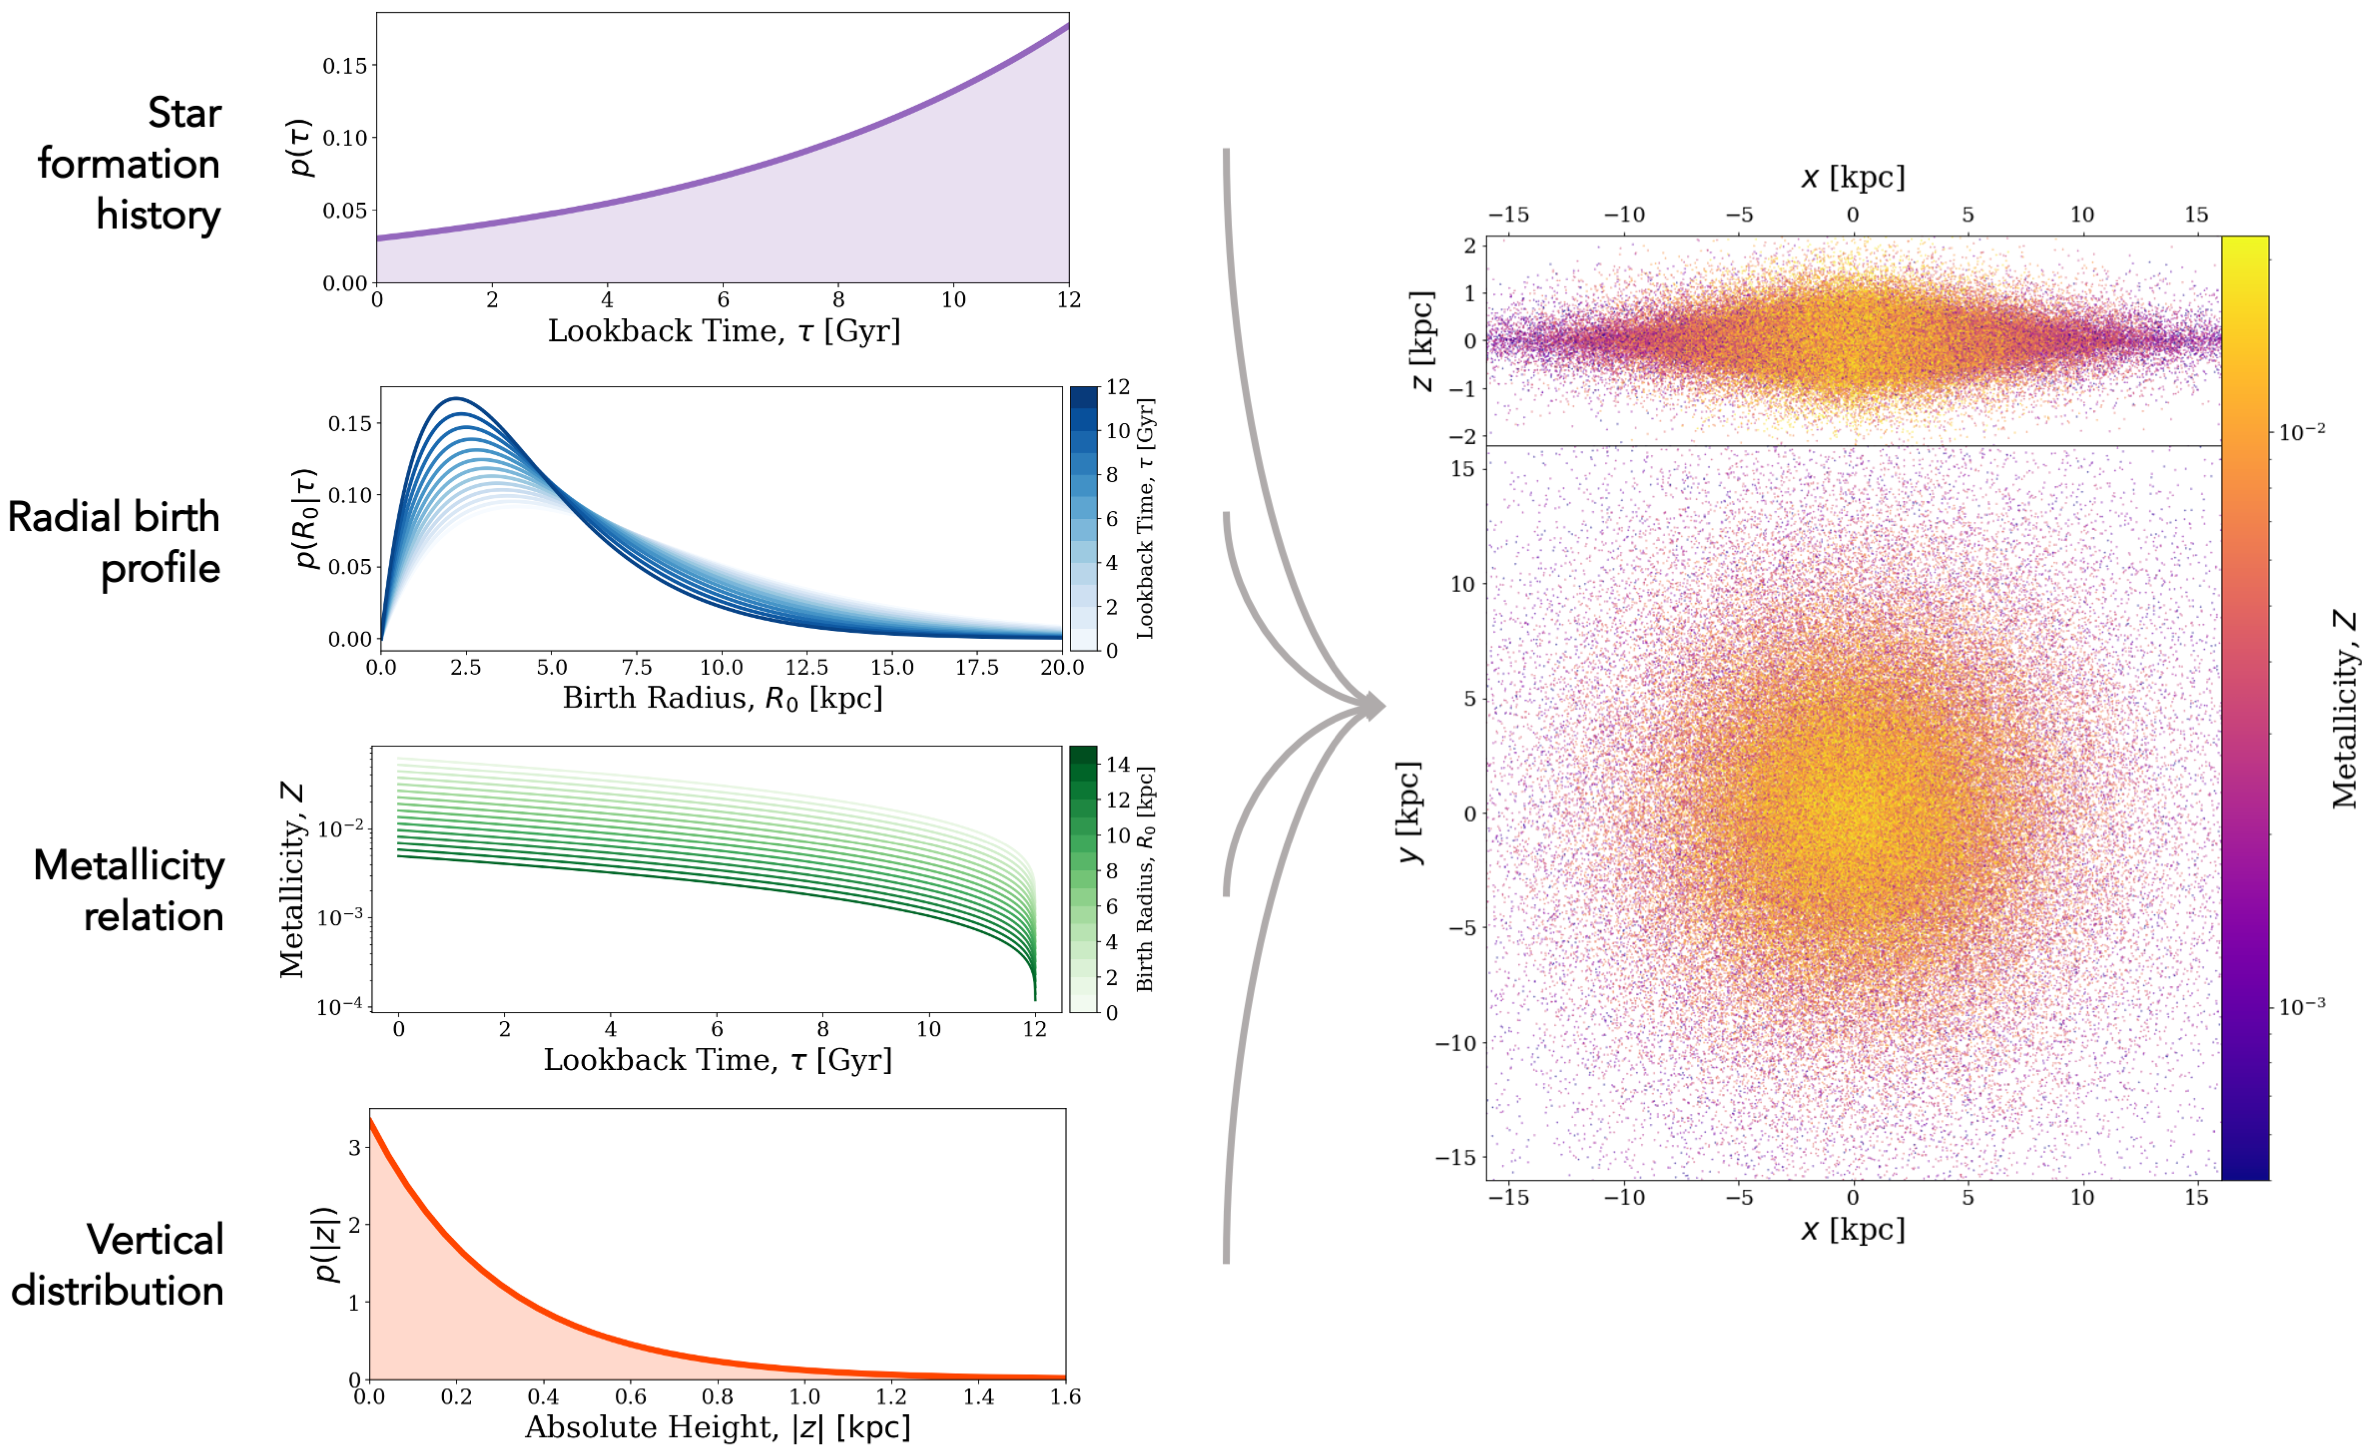
\includegraphics[width=\textwidth]{galaxy_diagram.png}
    \caption{A schematic showing how we create a mock Milky Way disc. On the left, we show the various distributions presented in \citet{Frankel+2018} and \citet{McMillan+2011}. On the right, we show an example instance of the Milky Way with $10^5$ binaries shown as points. The colour of each point represents its metallicity (with $Z \in [0.0001, 0.022]$). The top panel shows a side-on view and the bottom panel shows a view from above.}
    \label{fig:galaxy_schematic}
\end{figure*}

% \begin{figure}[t]
%     \centering
%     \includegraphics[width=\columnwidth]{galaxy_metallicity.png}
%     \caption{A random instance of the Milky Way of $10^5$ binaries, created using distributions from \citet{Frankel+2018}. The colour of each point represents its metallicity (with $Z \in [0.0001, 0.022]$). The top panel shows a side-on view and the bottom panels shows a view from above.}
%     \label{fig:galaxy_metallicity}
% \end{figure}

We match each set of galaxy parameters $\mathbf{g}_{{i}}$, to a random set of binary parameters $\mathbf{b}_{{Z, i}}$, by randomly drawing a set of binary parameters from the closest metallicity bin to the metallicity in $\mathbf{g}_{{i}}$.

Each binary is likely to move from its birth orbit. Although all stars in the Galactic disc experience some amount of radial migration \citep{Sellwood+2002, Frankel+2018}, double compact objects generally experience stronger dynamical evolution as a result of the effects of both Blaauw kicks from instantaneous symmetric mass loss \citep{Blaauw+1961} and natal kicks from asymmetric supernovae \citep{Hobbs+2005}.

The magnitude of the systemic kicks are typically small compared to the intital circular velocity of a binary at each Galactocentric radius. Therefore, kicks will not significantly alter the overall distribution of their positions. Given this, and for the sake of computational efficiency, we do not account for the displacement due to systemic kicks in our analysis.

\subsection{Gravitational Wave Inspiral}

Each binary loses orbital energy to gravitational waves throughout its lifetime. This causes the binary to shrink and circularise over time. In order to assess the detectability of a binary, we need to know its eccentricity and frequency at the time of the LISA mission. For each binary in our simulated Milky Way, we know that the time from DCO formation to today is $\tau - t_{\rm evolve}$ and that the initial eccentricity and semi-major axis are $e_{\rm DCO}$ and $a_{\rm DCO}$. We find the eccentricity of the binary at the start of the LISA mission, $e_{\rm LISA}$, by numerically integrating its time derivative \citep[][Eq. 5.13]{Peters+1964} given the initial conditions. This additionally can be converted to the semi-major axis at the start of LISA, $a_{\rm LISA} $\citep[][Eq. 5.11]{Peters+1964}, which in turn gives the orbital frequency, $f_{\rm orb, LISA}$, by Kepler's third law.

\subsection{Detectability}

We define a binary as detectable if its gravitational wave signal has a signal-to-noise ratio of greater than 7 \citep[e.g.][]{Breivik+2020, Korol+2020}. The sky-, polarisation- and orientation-averaged signal-to-noise ratio, $\rho$, of an inspiraling binary can be calculated with the following\footnote{For full derivations of the equations in this section, please see Appendix \ref{app:strain_snr_deriv}.} \citep[e.g.][]{Finn+2000}
\begin{equation}\label{eq:snr}
    \rho^2 = \sum_{n=1}^{\infty} \int_{f_{n, i}}^{f_{n, f}} \frac{h_{c, n}^{2}}{f_{n}^{2} S_{\rm n}\left(f_{n}\right)} \dd{f_n},
\end{equation}
where $n$ is a harmonic of the gravitational wave signal, $f_n = n \cdot f_{\rm orb}$ is the frequency of the $n^{\rm th}$ harmonic of the gravitational wave signal, $f_{\rm orb}$ is the orbital frequency, $S_{\rm n}(f_n)$ is the LISA sensitivity curve at frequency $f_n$ \citep[e.g.][]{Robson+2019} and $h_{c,n}$ is the characteristic strain of the $n^{\rm th}$ harmonic, given by
\begin{equation}\label{eq:charstrain}
    h^2_{c,n} = \frac{2^{5/3}}{3 \pi^{4/3}} \frac{(G \mathcal{M}_c)^{5/3}}{c^3 D_L^2} \frac{1}{n f_{\rm orb}^{1/3}} \frac{g(n,e)}{F(e)}
\end{equation}
\citep[e.g.][]{Barack+2004}, where $D_L$ is the luminosity distance to the source, $f_{\rm orb}$ is the orbital frequency, $g(n, e)$ and $F(e)$ are given in \citet{Peters+1963} and $\mathcal{M}_c$ is the chirp mass, defined as
\begin{equation}\label{eq:chirp_mass}
    \mathcal{M}_c = \frac{(m_1 m_2)^{3/5}}{(m_1 + m_2)^{1/5}}.
\end{equation}

For the sake of computational efficiency, it is convenient to make the approximation that many of the binaries are stationary in frequency space on the timescale of the observing mission. This simplifies the signal-to-ratio equation to
\begin{equation}\label{eq:snr_stat}
    \rho_{\rm stat}^2 = \sum_{n=1}^{\infty} \frac{2 \, T_{\rm obs} h_n^2}{S_n(f_n)},
\end{equation}
where $T_{\rm obs}$ is the observing time and $h_n$ is the strain amplitude of gravitational waves emitted in the $n^{\rm th}$ harmonic, given by
\begin{equation}
    h_n^2 = \frac{2^{25/3}}{5} \frac{\left(G \mathcal{M}_{c}\right)^{10/3}}{c^{8}} \frac{\left(\pi f_{\mathrm{orb}}\right)^{4 / 3}}{D_L^2} \frac{g(n, e)}{n^2}.
\end{equation}

We consider a binary as stationary if its change in gravitational wave frequency is less than 1\% of the initial frequency. None binaries in our sample are in the non-stationary regime and therefore we believe that this is an acceptable approximation.

\subsection{Detection rate}
We calculate the detection rate for any one Milky Way instance by determining the fraction of binaries that are detectable and normalising to the true mass and IMF of the Milky Way in order to account for our relatively smaller galaxy size and restricted mass ranges. For a more in-depth discussion of this normalisation process see Appendix~\ref{app:rate_normalisation}.

%%%%%%%%%%%%%%%%%%%%%%%%%%%%%%%%%%%%%%%%
%%%%%%%%%%%%%%%%%%%%%%%%%%%%%%%%%%%%%%%%
\section{Results (I)  - Survey of the Problem} \label{sec:resultsI}
%%%%%%%%%%%%%%%%%%%%%%%%%%%%%%%%%%%%%%%%
%%%%%%%%%%%%%%%%%%%%%%%%%%%%%%%%%%%%%%%%

In this section, we explore the problem of detecting double compact objects with LISA analytically, focussing specifically on BHNS binaries, before presenting our full simulation results in Section~\ref{sec:resultsII}.

\subsection{The Role of Eccentricity}\label{sec:eccentricity_role}

Unlike BHBH binaries, a significant fraction of the BHNS binary population is highly eccentric. A high eccentricity has two major effects on detecting a binary with gravitational waves.

Firstly, eccentricity enhances the rate of energy emission via gravitational waves by a factor
\begin{equation}
    F(e) = \frac{1 + (73 / 24) e^2 + (37 / 96) e^4}{(1 - e^2)^{7/2}},
\end{equation}
compared to a circular binary with the same semi-major axis \citep[][Eq.\,17]{Peters+1963}. This means that eccentric binaries will not only inspiral faster, but also produce gravitational waves with stronger strain amplitudes (when summed over all harmonics).

Secondly, eccentric binaries will emit gravitational waves at many harmonic frequencies (unlike circular binaries, which only emit at twice the orbital frequency). This leads to the gravitational wave signal being diluted over many frequencies higher than the orbital frequency, where the higher the eccentricity, the more harmonics are required to capture all of the gravitational luminosity \citep[see][Fig.\,3]{Peters+1963}.

Therefore, though the first effect always increases the strength of the signal, the two effects in tandem do not necessarily always increase the detectability of a binary and we illustrate this point in Fig.\,\ref{fig:ecc_effects}. We show effect of eccentricity on the gravitational wave signal from a typical BHNS binary of chirp mass $\mathcal{M}_c = 3 \unit{M_{\odot}}$ and distance $8 \unit{kpc}$ at an orbital frequency of $f_{\rm orb} = 3 \times 10^{-4} \unit{Hz}$. Increasing the eccentricity from $e = 0.0$ to $0.5$ results in an increase in the signal-to-noise ratio (annotated on each set of points). This is because the eccentricity not only increases the gravitational wave emission, but also shifts the peak of the signal towards the minimum of the LISA sensitivity curve. However, further increasing the eccentricity from $e = 0.5$ to $0.9$ instead \textit{decreases} the signal-to-noise ratio. Although the greater eccentricity produces a stronger strain, it also shifts the peak of the gravitational wave signal to such high frequencies that the noise level is much higher and therefore has a lower signal-to-noise ratio.

Overall, we can therefore conclude that for BHNS binaries, higher eccentricity will produce more detectable binaries only if the orbital frequency is not already at or above the minimum of the LISA sensitivity curve. Another consideration for more massive binaries is whether the increased eccentricity will cause the binary to merge before the mission ends, which would cause a significant decrease in signal-to-noise ratio.

\begin{figure}[htb]
    \centering
    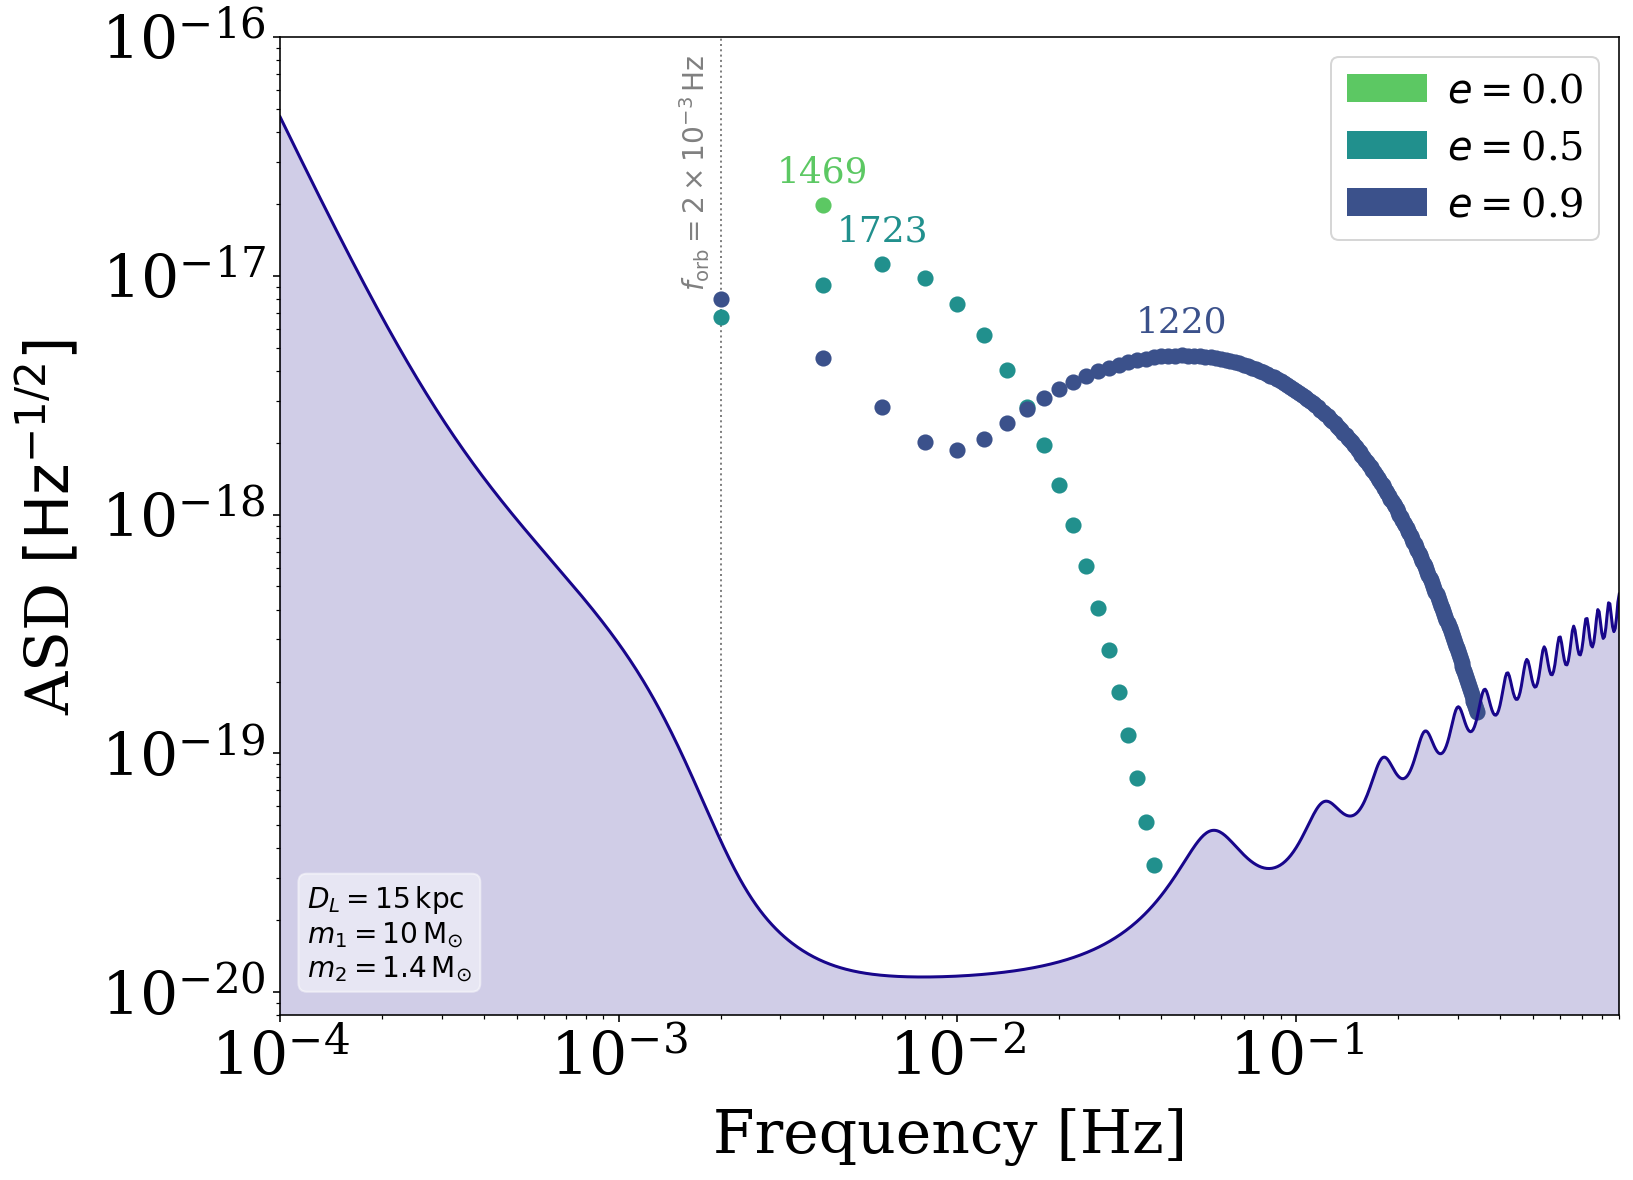
\includegraphics[width=\columnwidth]{e_sc_combined.png}
    \caption{An illustration of the effect of eccentricity on the detectability of a typical BHNS binary. Each point shows the strength of the gravitational wave signal at a harmonic frequency. We annotate each set of points with the binary's total signal-to-noise ratio summed over all harmonics and overplot the LISA sensitivity curve \citep{Robson+2019}.}
    \label{fig:ecc_effects}
\end{figure}

\subsection{Horizon Distance}

We define the horizon distance as the maximum distance at which a binary will have an signal-to-noise ratio above 7. In Figure~\ref{fig:bhns_horizon_distance} we show the horizon distance for a typical BHNS binary for different orbital frequencies and eccentricities. The horizon distance increases with frequency since the signal-to-noise ratio scales as
\begin{equation}
    \rho \propto \frac{N_{\rm cycle} \cdot h}{S_{\rm n}(f)} \propto \frac{f^{2/3} \cdot f^{1/2}}{S_{\rm n}(f)} \propto \frac{f^{7/6}}{S_{\rm n}(f)}.
\end{equation}
Since the minimum in the sensitivity curve occurs at $f \sim 10^{-2} \unit{Hz}$, the horizon distance increases monotonically with frequency. The dependence of the horizon distance on eccentricity follows the trends that we outlined in Section~\ref{sec:eccentricity_role}. The horizon distance increases with eccentricity up to a maximum, before decreasing once the eccentricity moves the peak of the gravitational wave luminosity past the minimum of the sensitivity curve. The eccentricity at which this maximum occurs is lower for higher orbital frequencies as less eccentricity is needed to move the peak past the minimum in the sensitivity curve. One may also note the sharp decrease in the horizon distance for binaries to the right of the $T_{\rm obs}$ contour, since these binaries will merge before the LISA mission is over.

This plot shows that, in principle, we could detect a BHNS binary up to several Mpc from Earth and thus plausibly in any galaxy in the Local Group. In reality, the number extragalactic detections will likely be very low since the binary needs to be very close to merging to be visible at that distance (as can be noted from the inspiral contours in Fig.~\ref{fig:bhns_horizon_distance}) and it is unlikely that a binary happen to be that close to merging during the LISA mission. However, more specific to this study, one can note that the combination of frequency and eccentricity required to be visible within the Milky Way (to the right of the white line in Fig.~\ref{fig:bhns_horizon_distance}) is much more probable.

\begin{figure}[htb]
    \centering
    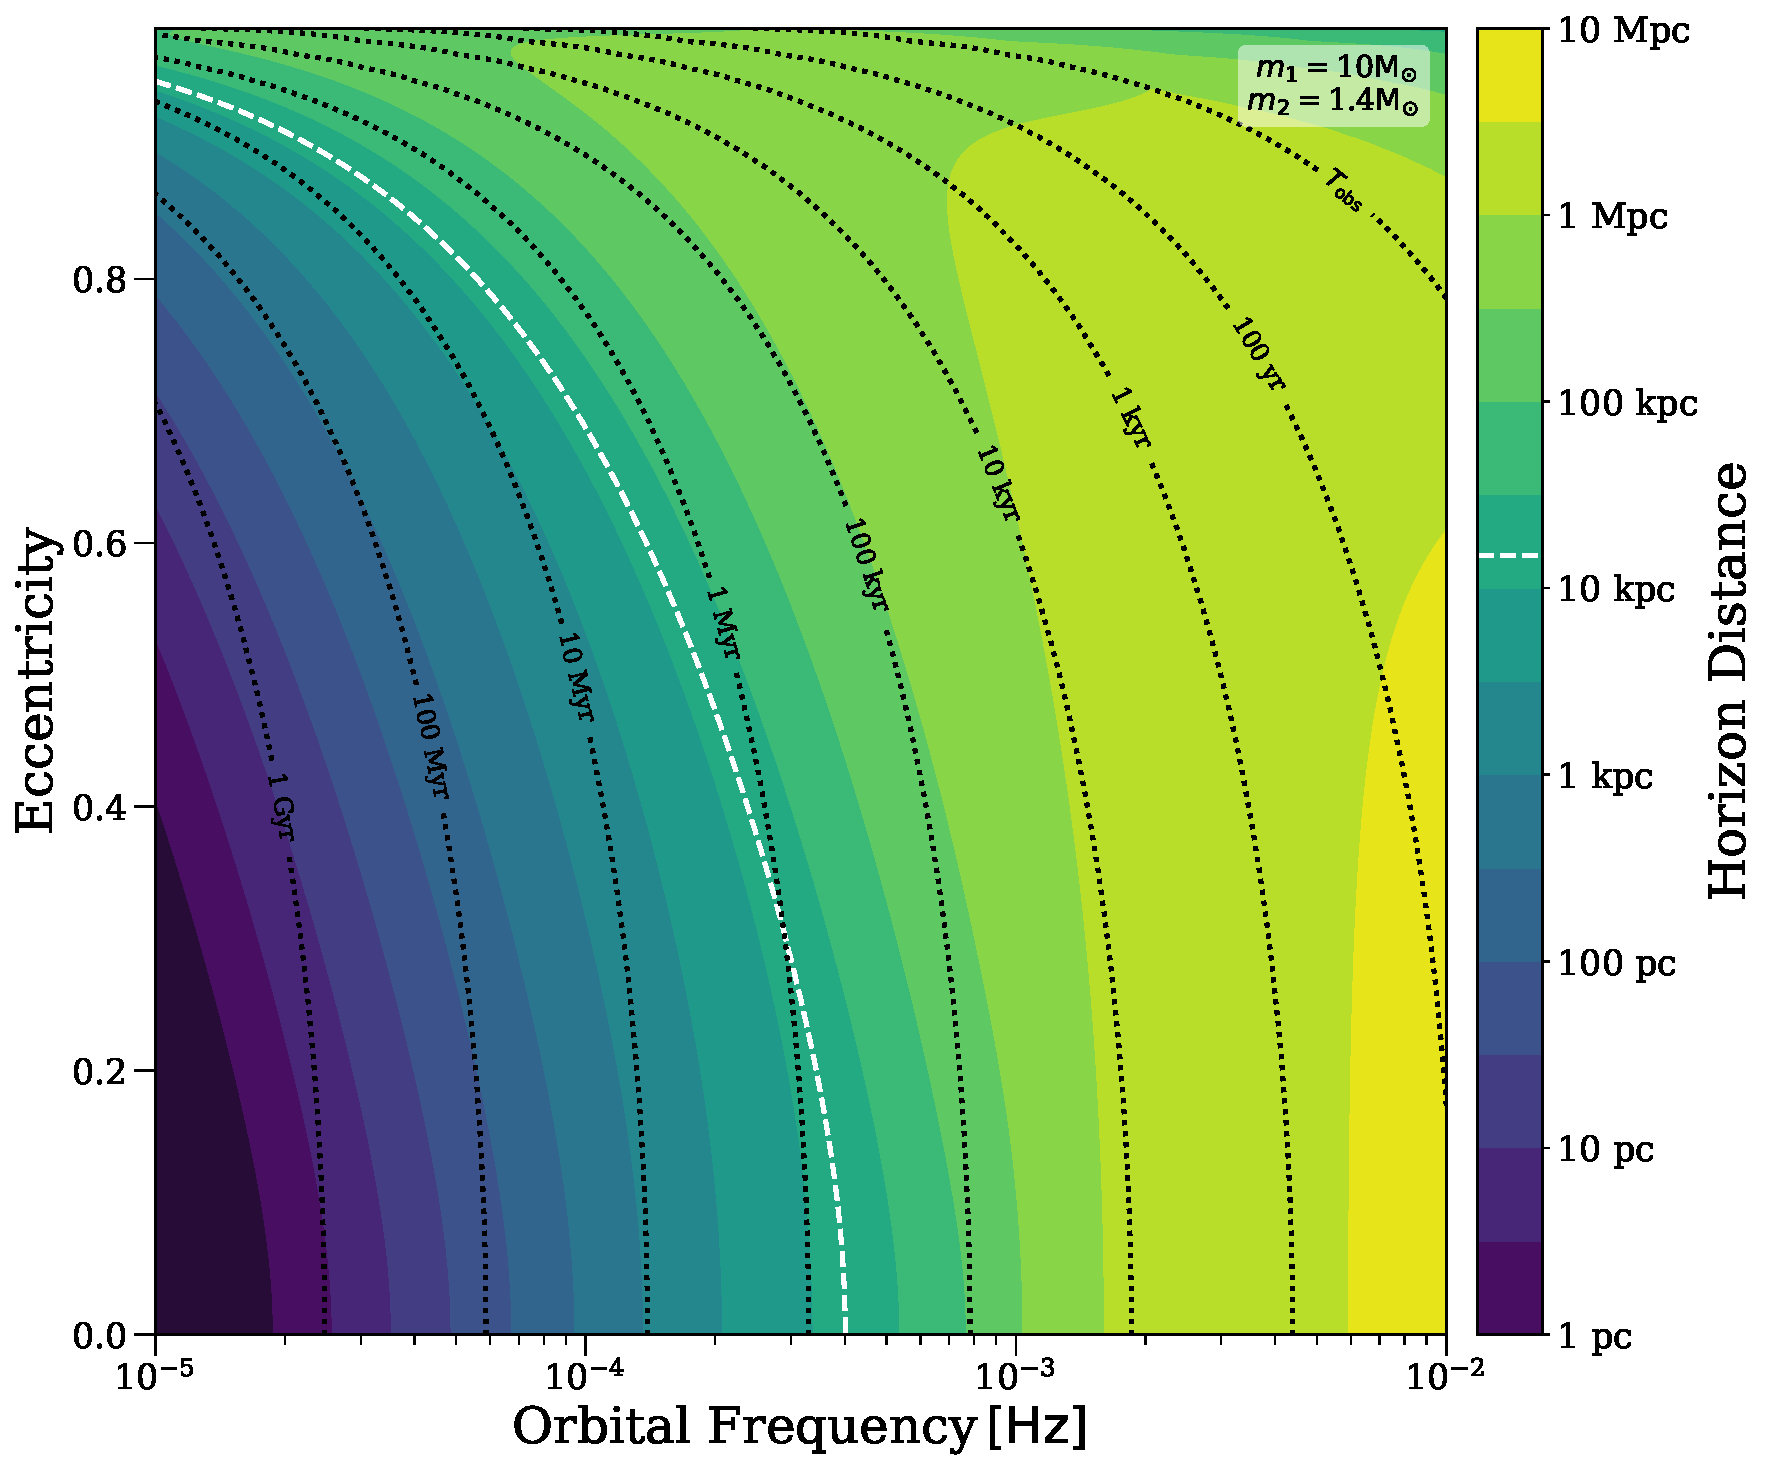
\includegraphics[width=\columnwidth]{horizon_distance.pdf}
    \caption{The horizon distance for a typical BHNS binary at different initial orbital frequencies and eccentricities is shown in the filled contours. The dashed white line indicates the edge of the Milky Way when using the \cite{Frankel+2018} model, which we define as the distance within which 99\% of binaries are contained. The dotted black lines show the inspiral time for the binary.}
    \label{fig:bhns_horizon_distance}
\end{figure}

%%%%%%%%%%%%%%%%%%%%%%%%%%%%%%%%%%%%%%%%
%%%%%%%%%%%%%%%%%%%%%%%%%%%%%%%%%%%%%%%%
\section{Results (II) - Synthetic Galaxy} \label{sec:resultsII}
%%%%%%%%%%%%%%%%%%%%%%%%%%%%%%%%%%%%%%%%
%%%%%%%%%%%%%%%%%%%%%%%%%%%%%%%%%%%%%%%%

In Figure~\ref{fig:detection_rates}, we show the expected number of LISA detections for each model variation. We find that on average, for our fiducial model, a four year LISA mission will detect 26 BHBH, 27 BHNS and 11 NSNS binaries. Increasing the LISA mission length to ten years changes the number of detections to 42, 45 and 19 respectively. The BHBH detection rate is markedly robust across physics variations, with the expected detections in each model staying within 25\% of the fiducial rate (with the exception of model \modOpt{}). Thus even if there are changes in our understanding of the underlying physics before the LISA mission commences, the expected BHBH detection rate is unlikely to change significantly. In contrast, the NSNS and BHNS rates are very sensitive to changes in binary physics assumptions. Therefore, once LISA flies and we know the actual number of detections, we can compare to each model and possibly provide some constraint on binary evolution physics.

Here is some attempted reasoning about the trends:

\textbf{BHBH:} The major standout for the BHBHs is the optimistic. In this case Hertzsprung gap donors are allowed to survive CE and this is because many BHs are formed in this way rather than any effect on detectability. Can also comment on lower(higher) max NS mass being good(bad). Kicks same as BHNSs but less pronounced.

\textbf{BHNS:} Whole bunch of trends here. The decrease with increasing $\beta$ seems to be due to fewer BHNSs surviving CE events (since envelope is harder to eject). Floor explains this in her paper and also references Kruckow. optimistic higher same as BHBH. Rapid higher because BHBHs become BHNSs instead. Maximum neutron star masses affect things because: lower means more things become BH instead of NS hence fewer BHNS and vice versa. PISN doesn't affect this mass range. Lower kicks means fewer disruptions. No BH kick lower again because NS kick is main factor at that point. \todo{this leaves E, F, G todo}

\textbf{NSNS:} \todo{Why are B, C, D opposite?}. E is low because that's the main NSNS formation channel. CE follows nice trend (see Floor's about CE channels). Optimistic slightly up because duh. \todo{weirdly basically no change in rapid and max NS masses}. Lower kicks great as usual. No BH kicks no effect duh.

\begin{figure*}[p]
    \centering
    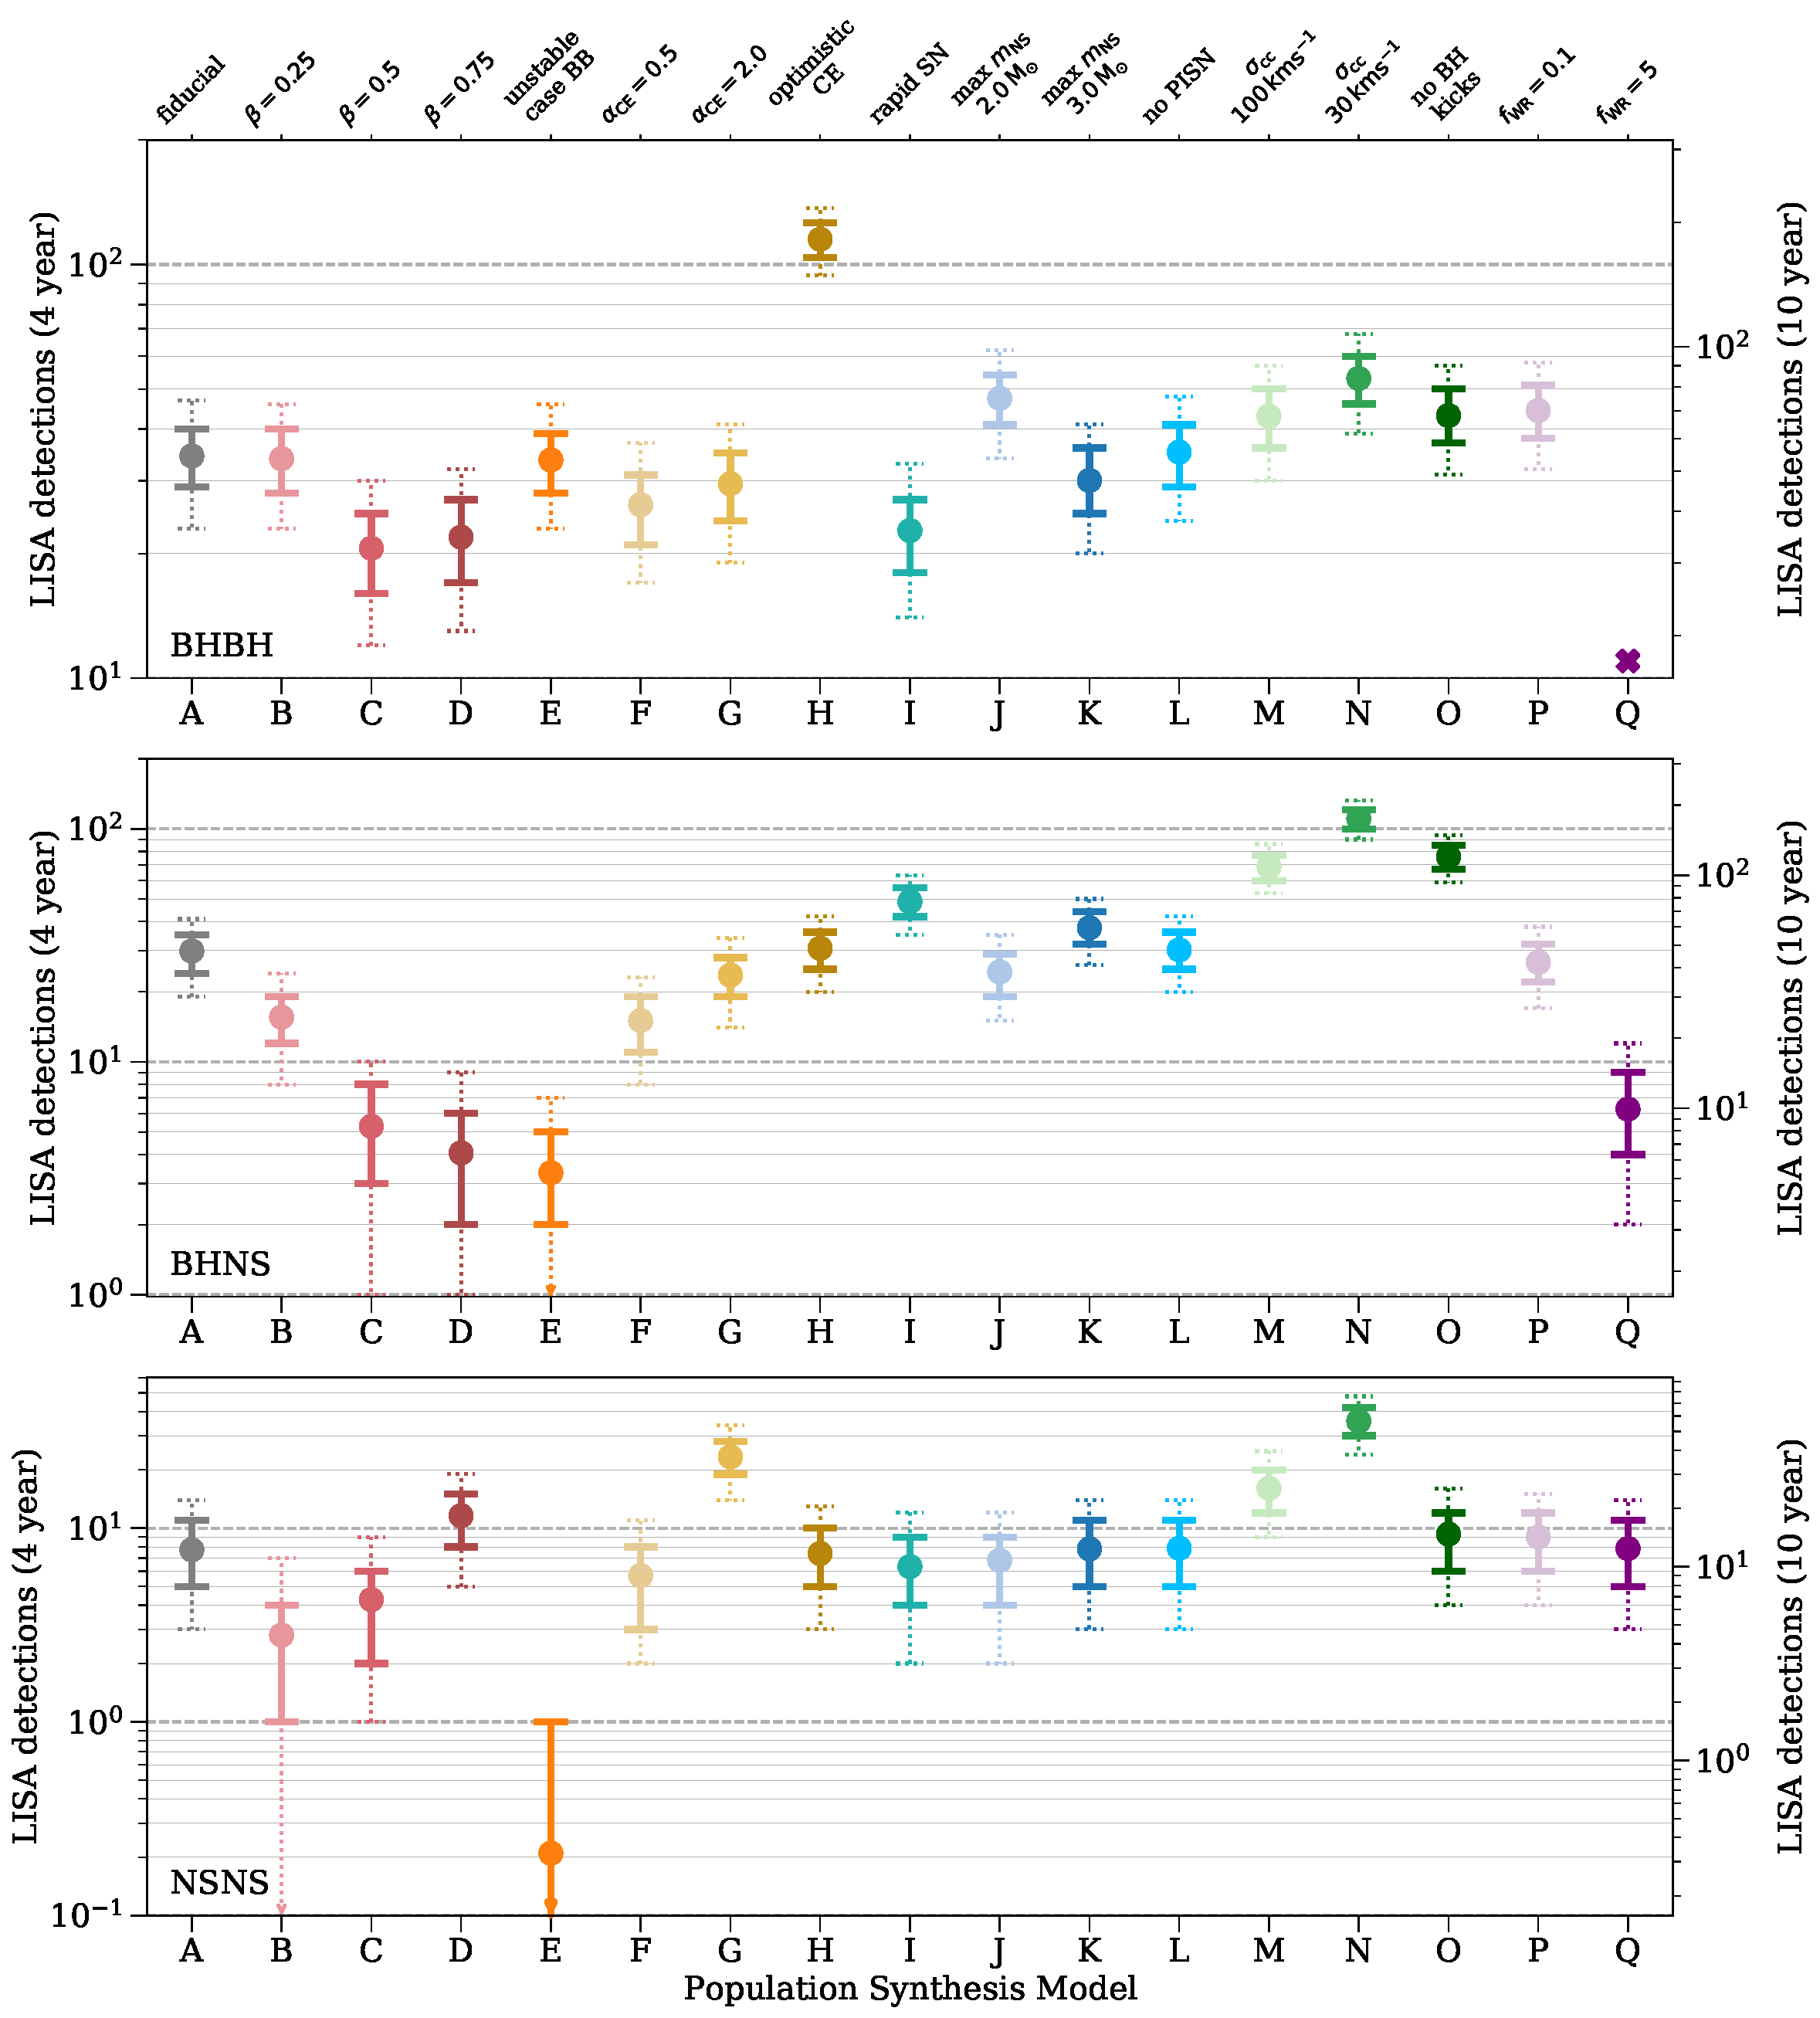
\includegraphics[width=\textwidth]{dco_detections.pdf}
    \caption{The number of expected detections in the LISA mission for different DCO types and model variations. Error bars show the 1 (solid) and 2 (dotted) $\sigma$ uncertainties. The left axis and grid lines show the number of detections in a four year LISA mission and the right axis shows an approximation of the number of detections in a 10 year mission (we scale the axis by $\sqrt{T_{\rm obs}}$, see Table~\ref{tab:detection_rates} for exact rates). Each model is described in further detail in Table~\ref{tab:physics_variations} and details of the fiducial assumptions are in  Section~\ref{sec:fiducial_physics}}
    \label{fig:detection_rates}
\end{figure*}

\begin{table*}[htb]
    \centering
    \caption{The number of detectable binaries in a 4 and 10 year LISA mission for the 15 different model variations and each DCO type. Each value shows the median and the 90\% confidence interval.}
    \begin{tabular}{c|lll|lll}
        \hline
        \multirow{2}{*}{Model} & \multicolumn{3}{c|}{LISA (4 year)} & \multicolumn{3}{c}{LISA (10 year)} \\ \cline{2-7}
         & \scriptsize{BHBH} & \scriptsize{BHNS} & \scriptsize{NSNS} & \scriptsize{BHBH} & \scriptsize{BHNS} & \scriptsize{NSNS} \\
        \hline
        A & \confinv{25.9}{11.1}{13.6} & \confinv{26.7}{11.9}{14.8} & \confinv{11.3}{6.4}{8.0} & \confinv{42.0}{17.3}{17.3} & \confinv{44.5}{17.8}{20.7} & \confinv{19.3}{8.0}{9.7}\\
        B & \confinv{27.7}{12.6}{12.6} & \confinv{12.0}{6.0}{7.5} & \confinv{4.7}{2.7}{3.3} & \confinv{42.7}{17.6}{17.6} & \confinv{19.5}{7.5}{10.5} & \confinv{8.0}{3.3}{4.0}\\
        C & \confinv{20.6}{9.4}{11.3} & \confinv{6.2}{2.8}{3.4} & \confinv{5.5}{2.7}{4.1} & \confinv{33.8}{13.1}{13.1} & \confinv{10.1}{3.9}{3.9} & \confinv{9.6}{4.1}{4.1}\\
        D & \confinv{20.0}{8.3}{10.0} & \confinv{3.2}{1.6}{1.6} & \confinv{14.6}{8.3}{10.4} & \confinv{31.7}{11.7}{11.7} & \confinv{5.1}{1.9}{2.2} & \confinv{22.9}{10.4}{12.5}\\
        E & \confinv{24.4}{12.2}{14.7} & \confinv{6.8}{3.8}{3.8} & \confinv{0.2}{0.1}{0.1} & \confinv{41.5}{17.1}{17.1} & \confinv{10.6}{3.8}{5.3} & \confinv{0.4}{0.1}{0.2}\\
        F & \confinv{20.0}{10.0}{10.0} & \confinv{11.5}{6.6}{8.2} & \confinv{8.1}{3.6}{5.4} & \confinv{30.0}{12.0}{14.0} & \confinv{19.7}{9.9}{9.9} & \confinv{13.6}{5.4}{6.3}\\
        G & \confinv{25.7}{9.9}{13.8} & \confinv{23.3}{10.6}{10.6} & \confinv{26.5}{15.1}{18.9} & \confinv{39.5}{13.8}{15.8} & \confinv{36.1}{12.7}{17.0} & \confinv{45.4}{18.9}{22.7}\\
        H & \confinv{63.6}{31.8}{47.7} & \confinv{37.4}{20.8}{20.8} & \confinv{14.7}{8.4}{10.5} & \confinv{103.4}{39.8}{55.7} & \confinv{62.3}{24.9}{29.1} & \confinv{25.2}{12.6}{12.6}\\
        I & \confinv{21.7}{10.9}{13.0} & \confinv{56.8}{31.6}{31.6} & \confinv{11.0}{5.5}{6.9} & \confinv{32.6}{13.0}{15.2} & \confinv{94.7}{37.9}{44.2} & \confinv{17.9}{8.3}{8.3}\\
        J & \confinv{32.6}{16.3}{19.6} & \confinv{20.3}{9.0}{13.5} & \confinv{11.0}{6.3}{7.8} & \confinv{52.2}{19.6}{22.8} & \confinv{33.8}{11.3}{15.8} & \confinv{18.8}{7.8}{9.4}\\
        K & \confinv{21.4}{9.7}{11.7} & \confinv{30.6}{13.6}{17.0} & \confinv{11.5}{6.6}{8.2} & \confinv{35.0}{13.6}{15.6} & \confinv{51.1}{20.4}{23.8} & \confinv{19.8}{8.2}{9.9}\\
        L & \confinv{24.7}{9.9}{14.8} & \confinv{26.7}{14.8}{17.8} & \confinv{11.3}{6.4}{8.0} & \confinv{42.0}{14.8}{17.3} & \confinv{44.5}{17.8}{20.7} & \confinv{19.3}{8.0}{9.7}\\
        M & \confinv{29.7}{13.2}{16.5} & \confinv{70.6}{39.2}{39.2} & \confinv{20.4}{11.7}{11.7} & \confinv{46.1}{19.8}{23.1} & \confinv{109.8}{39.2}{54.9} & \confinv{32.1}{14.6}{17.5}\\
        N & \confinv{31.6}{15.8}{19.7} & \confinv{117.7}{58.8}{73.6} & \confinv{51.8}{29.6}{29.6} & \confinv{51.3}{23.7}{23.7} & \confinv{191.3}{73.6}{103.0} & \confinv{81.4}{37.0}{44.4}\\
        O & \confinv{30.2}{15.1}{18.9} & \confinv{96.7}{48.3}{60.4} & \confinv{11.4}{6.5}{8.1} & \confinv{49.1}{22.7}{22.7} & \confinv{157.1}{60.4}{84.6} & \confinv{19.5}{9.7}{9.7}\\
        \hline
    \end{tabular}
    \label{tab:detection_rates}
\end{table*}


Now talk about where they are on the sensitivity curve

We illustrate the distribution of detectable DCOs on the sensitivity curve in Figure~\ref{fig:dcos_on_sc}. The shape of the distributions are bounded by the edge of the Milky Way and the scarcity of nearby DCOs. We indicate this with lines of constant distance that form as a boundary for the majority of DCOs, where the remaining scatter is due to variations in mass since lines are plotted for the average chirp mass of each respective DCO. The top edge is not a hard cutoff but is present because for any given distance there is a lower probability of drawing higher frequencies (since binaries spend more time at lower frequencies).

\begin{figure*}[t]
    \centering
    \includegraphics[width=\textwidth]{dcos_on_sc.png}
    \caption{Density distribution of detectable DCOs plotted over the LISA sensitivity curve \citep{Robson+2019}. We plot the total signal of binaries at their dominant frequency $n f_{\rm orb}$, such that $n$ is the harmonic that produces the most relative gravitational wave luminosity ($n = 2$ for circular binaries). If the density of points is below our lowest contour (2\%) then we plot the points as scatter points, where their sizes corresponds to their STROOPWAFEL weights. In order to explain the edges of the distribution, we additionally plot lines of constant distance. The dotted lines show the signal for a circular binary of average chirp mass, whilst the dashed line shows the signal for a binary with $e = 0.9$}
    \label{fig:dcos_on_sc}
\end{figure*}


\subsection{Distributions for the fiducial model}\label{sec:fiducial_distributions}

In Figure~\ref{fig:fiducial_pdf_distributions}, we show the distribution of the individual parameters of the population of detectable binaries and discuss the various features in the following sections.

\subsubsection{Black Hole Mass}
For both the BHBHs and BHNSs, the black hole mass distribution extends across relatively low masses, with $83\%$ and $90\%$ respectively below $10 \unit{M_{\odot}}$. This is because, at the high metallicities in the Milky Way, stellar winds are much stronger and strip away much of the stellar mass before BH formation. The mass distribution also extends down to $2.5 \unit{M_{\odot}}$, our fiducial maximum neutron star mass, since the \citet{Fryer+2012} \textit{delayed} remnant mass prescription does not produce a mass gap between neutron stars and black holes. Thus BHBHs and BHNSs detected by LISA could be ideal for ascertaining whether there exists a lower mass gap between neutron stars and black holes.

The bimodality of the BHBH distribution is a result of most detectable BHBHs in our sample having unequal mass ratios. The two peaks are from the primary and secondary black hole masses and we show their individual distributions with the dotted curves.

The reasoning for these unequal mass ratio is as follows: in order to produce a BHBH, most formation channels require at least the first mass transfer to be stable. This stability is strongly dependent on the mass ratio such that equal mass ratios (at the moment of mass transfer) are preferred for creating BHBHs. Yet, since stellar winds are so strong at high metallicity, and even stronger for more massive stars, the primary star will experience significant mass loss and so an initially \textit{unequal} mass ratio is preferred so that the masses are more balanced at the first instance of mass transfer. Since mass transfer occurs after the end of the main sequence for most of our BHBHs, the star will have a well defined core and these core masses, which go on to form BHs, will reflect the initially unequal mass ratios.

\subsubsection{Neutron Star Mass}
The neutron star mass distribution shows that most neutron stars have low masses, with $69\%$ and $87\%$ having masses below $1.5 \unit{M_{\odot}}$ for BHNSs and NSNSs respectively. The lacks of neutron stars around $1.7 \unit{M_{\odot}}$ and the subsequent small peaks are artifacts of the discontinuous nature of the \citet{Fryer+2012} remnant mass prescription.

\subsubsection{Eccentricity}
The eccentricity distributions show that detectable BHBHs are the most eccentric of the three DCOs. This may seem counterintuitive since neutron stars receive stronger natal kicks, which cause the orbit to become eccentric. However, these stronger kicks often instead result in disrupted or too-wide binaries. In contrast, BHBHs can receive strong kicks that impart high eccentricity without disrupting and thus tend to be more eccentric. This effect is compounded by the fact that we can see BHBHs at lower orbital frequencies, meaning that they have not had as much time to circularise and so still have significant eccentricity by the time of the LISA mission.

\subsubsection{Orbital Frequency and Frequency Evolution}
The orbital frequency distributions for BHBHs, BHNSs and NSNSs peak at increasing frequencies. This is because a higher mass DCO at the same distance and eccentricity requires a lower frequency to produce the same signal-to-noise ratio and thus be detected. The BHBH distribution also has a tail that extends to $4 \times 10^{-6} \unit{Hz}$, which is comprised of highly eccentric binaries since eccentricity moves the dominant harmonic to higher frequencies. Similar tails are not as prevalent for BHNSs and NSNSs as they do not have as many eccentric binaries.

\subsubsection{Luminosity Distance}
Each DCO's luminosity distance distribution peaks around $8 \unit{kpc}$ since this is the distance to the centre of the Milky Way and thus the most dense location of DCOs. Each DCO also has a shoulder at lower distances since closer binaries are easier to detect. This shoulder is more prominent for the NSNS distribution since their lower relative masses require a smaller distance in order to be detected on average.

\subsubsection{Inspiral Time}
Each DCO has a strong peak at small inspiral times since higher metallicities lead to tighter binaries and thus shorter inspiral times. \todo{explain the bumps}

\begin{figure*}[htbp]
    \centering
    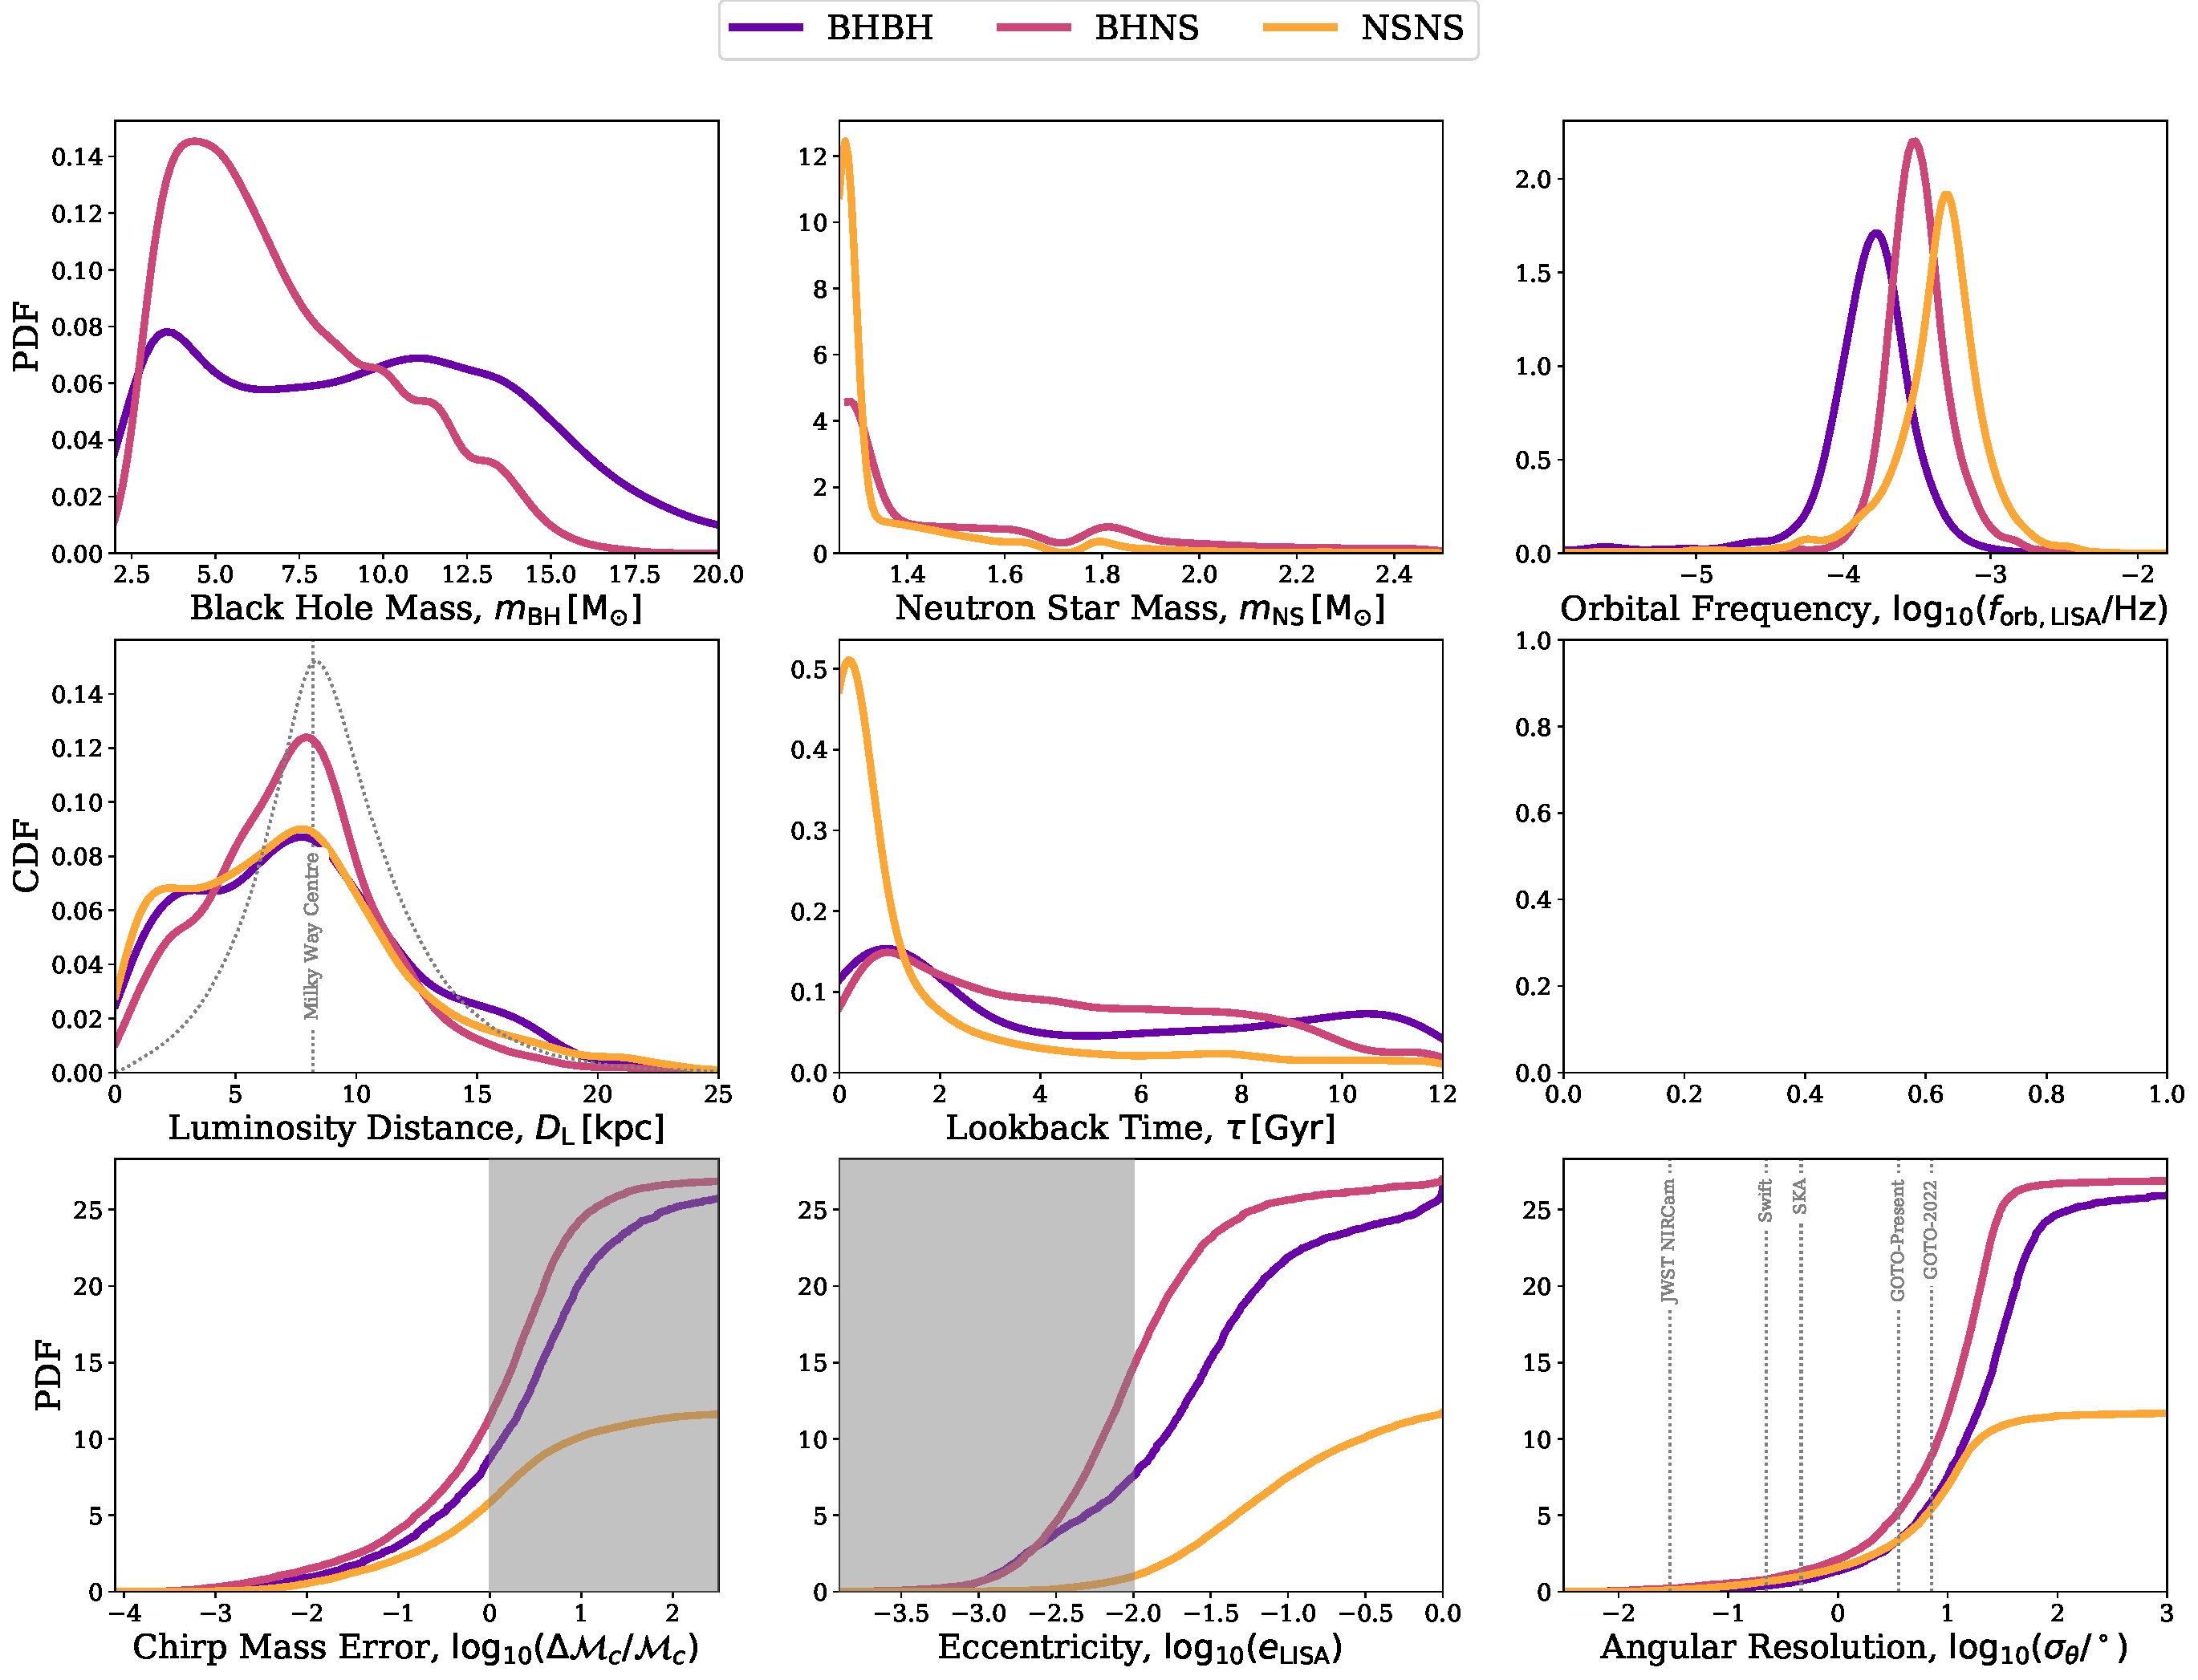
\includegraphics[width=\textwidth]{distribution_grid.pdf}
    \caption{Distributions for various parameters of the binaries that are detectable in a 4 year LISA mission in our fiducial model. Each line represents a kernel density estimator for the distribution and the colour denotes the double compact object type. The dotted curves in the black hole mass distribution show the primary and secondary mass distributions. In Section~\ref{sec:fiducial_distributions} we the features of the distributions.}
    \label{fig:fiducial_pdf_distributions}
\end{figure*}

\subsection{Distinguishing DCOs}
\todo{}

\begin{figure*}[htb]
    \centering
    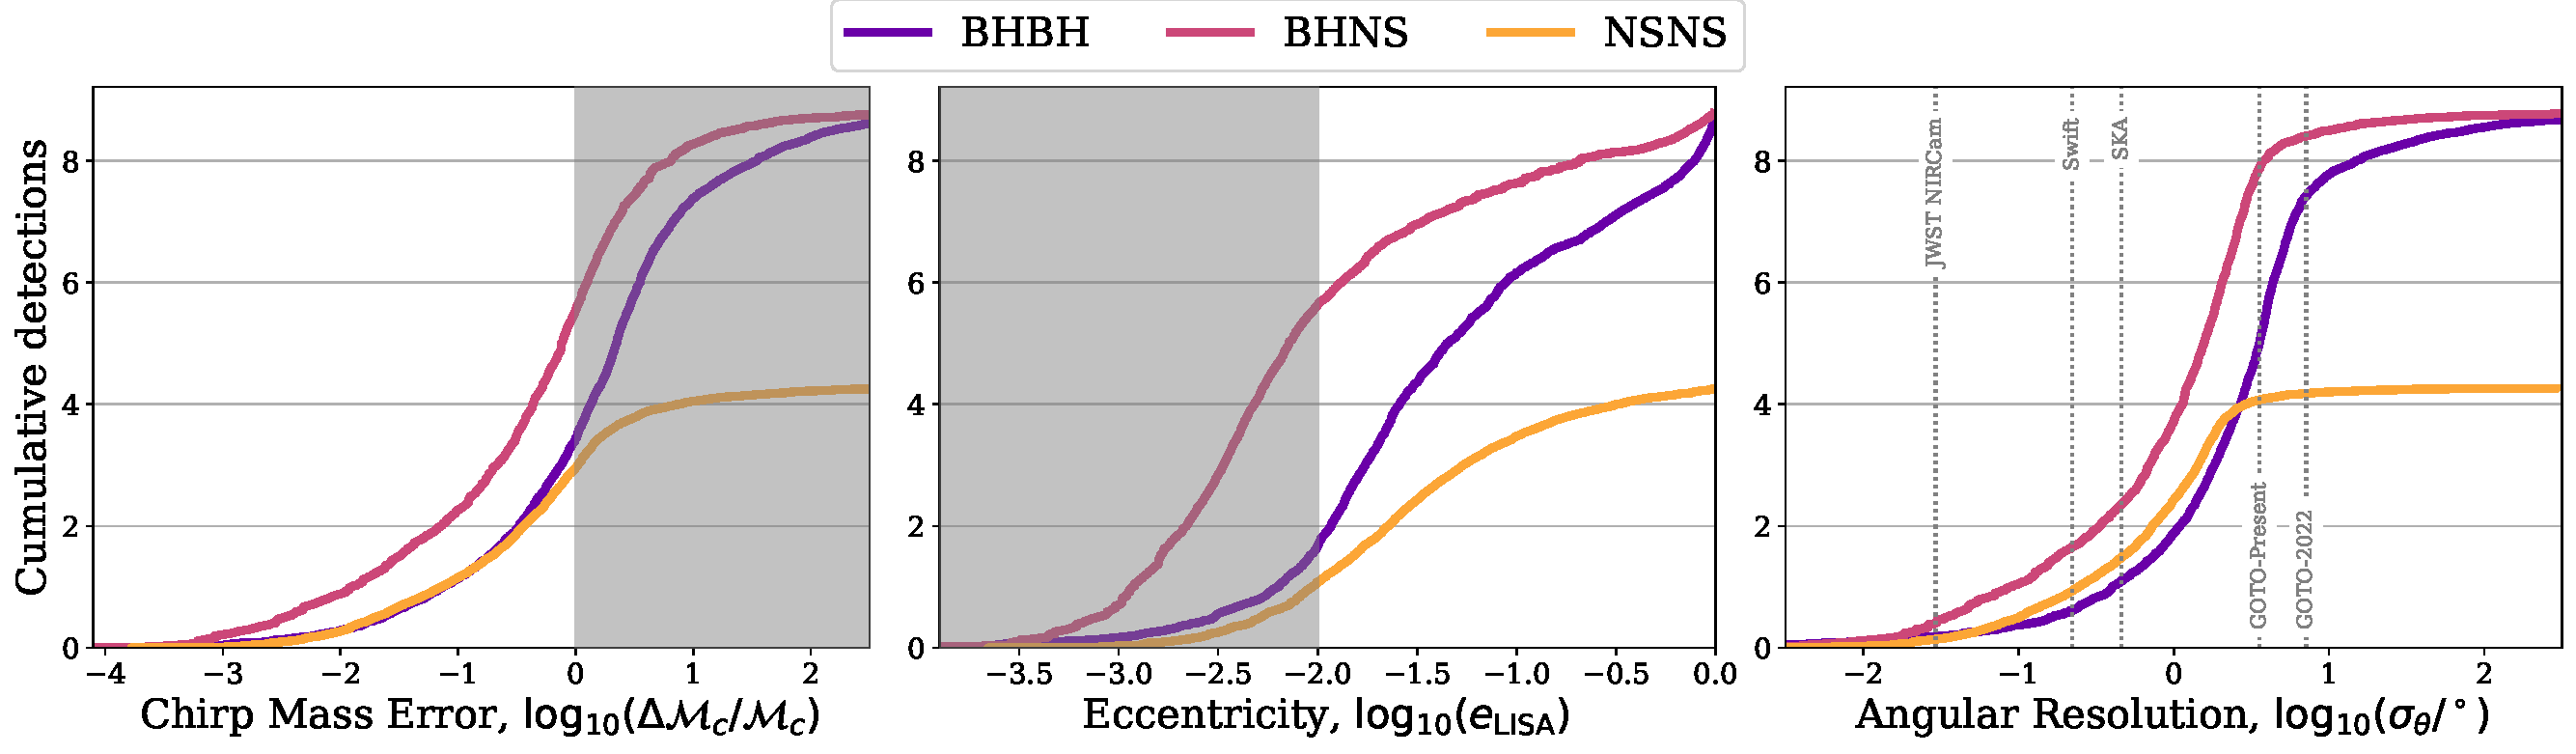
\includegraphics[width=\textwidth]{fiducial_cdf_distributions.pdf}
    \caption{Cumulative distributions of observable parameters for binaries that are detectable in a 4 year LISA mission. Shaded areas indicate regimes in which no measurement can be made. Dotted lines on the angular resolution distribution show the field of view for various telescopes that could perform EM counterpart observations.}
    \label{fig:fiducial_cdf_distributions}
\end{figure*}

\subsection{Model variations}


\subsection{Comparison with other studies}\label{sec:compare_studies}
\citet{Lau+2020} find that the number of NSNS binaries in the Milky Way that would be detected by a 4 year LISA mission is 33, a factor of three times higher than our fiducial rate. This study incorporates \citet{Lau+2020} uses the same population synthesis code, COMPAS, as this study, though an earlier version. They make several different physical assumptions, using the \citet{Fryer+2012} \textit{rapid} remnant mass prescription, limiting the maximum neutron star mass to $2 \unit{M_{\odot}}$ and not implementing PISN. However, we note that none of these assumptions significantly affect the NSNS LISA detection rate (see bottom panel of Fig.\,\ref{fig:detection_rates}, models \modRapid{}, \modNSLow{} and \modNoPISN{}).

We therefore surmise that the difference between our results is likely due to way in which we simulate the Milky Way. \citet{Lau+2020} assumes constant star formation, solar metallicity and distribute binaries following the blue light luminosity of the Milky Way, whilst we use the distributions from \citet{Frankel+2018} for the star formation rate, metallicity and positions. The \citet{Frankel+2018} star formation rate decreases over time and the metallicity distribution peaks above solar metallicity. Both of these changes could decrease the rate since most NSNS binaries in our sample have short inspiral times compared to the age of the Milky Way and higher metallicity would lead to increased stellar winds and hence less massive DCOs.

\citet{Breivik+2020} find that LISA will detect 93 BHBH, 33 BHNS and 8 NSNS binaries in the Milky Way over a 4 year mission. Although these are significantly different from our fiducial results, we make many different physical assumptions, the most notable being that \citet{Breivik+2020} assumes the optimistic CE scenario. Thus it would be more prudent to compare to our results from model \modOpt{} in which we find 70, 38 and 15 detections respectively. The discrepancy in the NSNS rate is likely due to the fact that we assume that case BB mass transfer onto a NS is always stable but \citet{Breivik+2020} does not and this would significantly decrease our rate (see bottom panel of Fig.\,\ref{fig:detection_rates}, model \modCaseBB{}) . The remaining differences are likely due to using a different population synthesis code (COSMIC) and using a different model for the Milky Way, particularly the assumptions of two fixed metallicities.

%%%%%%%%%%%%%%%%%%%%%%%%%%%%%%%%%%%%%%%%
%%%%%%%%%%%%%%%%%%%%%%%%%%%%%%%%%%%%%%%%
\section{Discussion} \label{sec:discussion}
%%%%%%%%%%%%%%%%%%%%%%%%%%%%%%%%%%%%%%%%
%%%%%%%%%%%%%%%%%%%%%%%%%%%%%%%%%%%%%%%%
\subsection{Caveats}
\begin{itemize}
    \item Standard pop synth limitations
    \item Systemic kicks
    \item No models for high $Z$ values in Frankel
    \item Only a single disc for the Milky Way
    \item Stationary approximation? But I'm pretty sure that is fine
\end{itemize}

\subsection{Can we distinguish them?}

\section{Conclusion \& Summary} \label{sec:conclusion}


%%%%%%%%%%%%%%%%%%%%%%%%%%%%%%%%%%%%%%%%
%%%%%%%%%%%%%%%%%%%%%%%%%%%%%%%%%%%%%%%%
%%%%%%%%%%%%%%%%%%%%%%%%%%%%%%%%%%%%%%%%
%%%%%%%%%%%%%%%%%%%%%%%%%%%%%%%%%%%%%%%%

\software{COMPAS (version 02.12.00) \url{http://github.com/TeamCOMPAS/COMPAS}. \citep{Stevenson+2017, Vigna-Gomez+2018, Broekgaarden+2019}, \texttt{Python} available from \url{python.org}, matplotlib \citep{Hunter+2007},  \texttt{NumPy} \citep{vanderWalt+2011}, 
Astropy \citep[\url{http://www.astropy.org}][]{AstropyCollaboration+2013, AstropyCollaboration+2018}.}

\acknowledgments{This project was funded in part by the European Union’s Horizon 2020 research and innovation program from the European Research Council (ERC, Grant agreement No. 715063), and by the Netherlands Organization for Scientific Research (NWO) as part of the Vidi research program BinWaves with project number 639.042.728. We further acknowledge the Black Hole Initiative funded by a generous contribution of the John Templeton Foundation and the Gordon and Betty Moore Foundation.}

\clearpage

\bibliographystyle{aasjournal}
\bibliography{references}

\allowdisplaybreaks

\appendix

\section{Derivation of Strain and SNR Equations}\label{app:strain_snr_deriv}
In this section we provide a full derivation/explanation of how we arrived at the equations used in our simulations.

\subsection{Conversions and definitions}
Each of these conversions and definitions are useful in the later derivations and we define them here for convenience. First, we define the chirp mass of a binary as 
\begin{equation}\label{eq:chirpmass}
    \mathcal{M}_c = \frac{(m_1 m_2)^{3/5}}{(m_1 + m_2)^{1/5}},
\end{equation}
where $m_1$ and $m_2$ are the primary and secondary mass of the binary. Kepler's third law is well known and allows one to convert between orbital frequency and the semi-major axis of a binary. For convenience we show it here
\begin{equation}\label{eq:kepler3rd}
    a = \qty(\frac{G(m_1 + m_2)}{(2 \pi f_{\rm orb})^{2}})^{1/3},\qquad f_{\rm orb} = \frac{1}{2 \pi} \sqrt{\frac{G(m_1 + m_2)}{a^3}}.
\end{equation}
As we deal with eccentric binaries, the different harmonic frequencies of gravitational wave emission become important. We therefore write that the relative power radiated into the $n^{\rm th}$ harmonic for a binary with eccentricity $e$ is \citep[][Eq.\,20]{Peters+1963}
\begin{equation}\label{eq:g(n,e)}
    \begin{aligned}
        g(n, e) = \frac{n^{4}}{32} & \left\{ \left[ J_{n-2}(n e)-2 e J_{n-1}(n e)+\frac{2}{n} J_{n}(n e)+2 e J_{n+1}(n e)-J_{n+2}(n e)\right]^{2}\right.\\
        &\left.+\left(1-e^{2}\right)\left[J_{n-2}(n e)-2 J_{n}(n e)+J_{n+2}(n e)\right]^{2}+\frac{4}{3 n^{2}}\left[J_{n}(n e)\right]^{2}\right\},
    \end{aligned}
\end{equation}
where $J_{n}(v)$ is the Bessel function of the first kind. Thus, the sum of $g(n, e)$ over all harmonics gives the factor by which the gravitational wave emission is stronger for a binary of eccentricity $e$ over an otherwise identical circular binary. This enhancement factor is defined by Peters as \citep[][Eq.\,17]{Peters+1963}
\begin{equation}\label{eq:eccentricity_enhancement_factor}
    F(e) = \frac{1 + (73 / 24) e^2 + (37 / 96) e^4}{(1 - e^2)^{7/2}}.
\end{equation}
Note that $F(0) = 1$ as one would expect. A fun number to remember is that $F(0.5) \approx 5.0$, or in words, a binary with eccentricity $0.5$ loses energy to gravitational waves at a rate $5$ times higher than a similar circular binary.

\subsection{Characteristic Strain}
The characteristic strain from a binary in the $n^{\rm th}$ harmonic is defined as follows (e.g. \citealp[][Eq.\,56]{Barack+2004}; \citealp[][Eq.\,5.1]{ Flanagan+1998})
\begin{equation}\label{eq:char_strain_dedf}
    h_{c,n}^2 = \frac{1}{(\pi D_L)^2} \qty( \frac{2 G}{c^3} \frac{\dot{E_n}}{\dot{f_n}} ),
\end{equation}
where $D_L$ is the luminosity distance to the binary, $\dot{E}_n$ is the power radiated in the $n^{\rm th}$ harmonic and $\dot{f}_n$ is the rate of change of the $n^{\rm th}$ harmonic frequency. The power radiated in the $n^{\rm th}$ harmonic is given by \citep[][Eq. 19]{Peters+1963}
\begin{equation}\label{eq:edot_peters}
    \dot{E}_n = \frac{32}{5} \frac{G^{4}}{c^5} \frac{m_{1}^{2} m_{2}^{2}\left(m_{1}+m_{2}\right)}{a^{5}} g(n, e),
\end{equation}
where $m_1$ is the primary mass, $m_2$ is the secondary mass, $a$ is the semi-major axis of the binary and $e$ is the eccentricity. Using \eqref{eq:chirpmass} and \ref{eq:kepler3rd}, we can recast \eqref{eq:edot_peters} in a form more applicable for gravitational wave detections that is a function of only the chirp mass, orbital frequency and eccentricity.
\begin{align}
    \dot{E}_n &= \frac{32}{5} \frac{G^{4}}{c^5} \qty(m_{1}^{2} m_{2}^{2}\left(m_{1}+m_{2}\right)) g(n, e) \cdot \qty(\frac{(2 \pi f_{\rm orb})^{2}}{G(m_1 + m_2)})^{5/3} \\
    \dot{E}_n &= \frac{32}{5} \frac{G^{7/3}}{c^5} \frac{m_{1}^{2} m_{2}^{2}}{\left(m_{1}+m_{2}\right)^{2/3}} (2 \pi f_{\rm orb})^{10/3} g(n, e) \\
    \dot{E}_n(\mathcal{M}_c, f_{\rm orb}, e) &= \frac{32}{5} \frac{G^{7 / 3}}{c^{5}}\left(2 \pi f_{\mathrm{orb}} \mathcal{M}_{c}\right)^{10 / 3} g(n, e) \label{eq:edot}
\end{align}
The last term needed to define the characteristic strain in \eqref{eq:char_strain_dedf} is the rate of change of the $n^{\rm th}$ harmonic frequency. We can first apply the chain rule and note that
\begin{equation}\label{eq:fdot_chainrule}
    \dot{f}_{n} = \dv{f_{n}}{a} \dv{a}{t}.
\end{equation}
The frequency of the $n^{\rm th}$ harmonic is simply defined as $f_n = n \cdot f_{\rm orb}$ and therefore we can find an expression for $\dd{f_{n}} / \dd{a}$ by rearranging and differentiating \eqref{eq:kepler3rd}
\begin{align}
    f_{n} &= \frac{n}{2 \pi} \sqrt{\frac{G(m_1 + m_2)}{a^3}}, \\
    \dv{f_{n}}{a} &= -\frac{3 n}{4 \pi} \frac{\sqrt{G(m_1 + m_2)}}{a^{5/2}}. \label{eq:dfda}
\end{align}
The rate at which the semi-major axis decreases is \citep[][Eq. 5.6]{Peters+1964}
\begin{equation}\label{eq:dadt}
    \dv{a}{t} = -\frac{64}{5} \frac{G^{3} m_{1} m_{2}\left(m_{1}+m_{2}\right)}{c^{5} a^{3}} F(e).
\end{equation}
Substituting \eqref{eq:dfda} and \ref{eq:dadt} into \eqref{eq:fdot_chainrule} gives an expression for $\dot{f}_{n}$
\begin{align}
    \dot{f}_n &= -\frac{3 n}{4 \pi} \frac{\sqrt{G(m_1 + m_2)}}{a^{5/2}} \cdot -\frac{64}{5} \frac{G^{3} m_{1} m_{2}\left(m_{1}+m_{2}\right)}{c^{5} a^{3}} F(e), \\
    \dot{f}_n &= \frac{48 n}{5 \pi} \frac{G^{7/2}}{c^5} \qty(m_1 m_2 (m_1 + m_2)^{3/2}) \frac{F(e)}{a^{11/2}},
\end{align}
which, as above with $\dot{E}_n$, we can recast using Kepler's third law and the definition of the chirp mass
\begin{align}
    \dot{f}_n &= \frac{48 n}{5 \pi} \frac{G^{7/2}}{c^5} \qty(m_1 m_2 (m_1 + m_2)^{3/2}) F(e) \cdot \qty(\frac{(2 \pi f_{\rm orb})^{2}}{G(m_1 + m_2)})^{11/6}, \\
    &= \frac{48 n}{5 \pi} \frac{G^{5/3}}{c^5} \frac{m_1 m_2}{(m_1 + m_2)^{1/3}} \cdot (2 \pi f_{\rm orb})^{11/3} \cdot F(e), \\
    \dot{f}_n(\mathcal{M}_c, f_{\rm orb}, e) &= \frac{48 n}{5 \pi} \frac{\qty(G \mathcal{M}_c)^{5/3}}{c^5} (2 \pi f_{\rm orb})^{11/3} F(e) \label{eq:fdot}
\end{align}
With definitions of both $\dot{E}_n$ and $\dot{f}_n$, we are now in a position to find an expression for the characteristic strain by plugging \eqref{eq:edot} and \ref{eq:fdot} into \ref{eq:char_strain}:
\begin{align}
    h^2_{c,n} &= \frac{1}{(\pi D_L)^2} \qty( \frac{2 G}{c^3} \frac{\frac{32}{5} \frac{G^{7 / 3}}{c^{5}}\left(2 \pi f_{\mathrm{orb}} \mathcal{M}_{c}\right)^{10 / 3} g(n, e)}{\frac{48 n}{5 \pi} \frac{\qty(G \mathcal{M}_c)^{5/3}}{c^5} (2 \pi f_{\rm orb})^{11/3} F(e)} ) \\
    &= \frac{1}{(\pi D_L)^2} \qty( \frac{2^{5/3} \pi^{2/3}}{3} \frac{(G \mathcal{M}_c)^{5/3}}{c^3} \frac{1}{f_{\rm orb}^{1/3}} \frac{g(n, e)}{n F(e)} ) \\
    h_{c,n}^2(\mathcal{M}_c, D_L, f_{\rm orb}, e) &= \frac{2^{5/3}}{3 \pi^{4/3}} \frac{(G \mathcal{M}_c)^{5/3}}{c^3 D_L^2} \frac{1}{f_{\rm orb}^{1/3}} \frac{g(n, e)}{n F(e)} \label{eq:char_strain}
\end{align}

\subsection{Strain}
The strain can be found by dividing the characteristic strain by the square root of twice the number of cycles. This is explained in \citet{Finn+2000} and in further detail in \citet{Moore+2015}. The physical reasoning behind the idea is that the binary will spend a certain amount of time in the vicinity of some frequency $f$ and cause a similar gravitational wave strain. This leads to the signal 'accumulating' and resulting in a larger signal-to-noise ratio. Therefore, the characteristic strain represents the strain measured by the detector over the duration of the mission, whilst the strain is what is emitted by the binary at each instantaneous moment.

Following this logic, we can convert between characteristic strain and strain with \citep[e.g][see text before Eq.\,2.2]{Finn+2000}
\begin{equation}\label{eq:strain-to-charstrain}
    h_{c, n}^2 = \qty(\frac{2 f_n^2}{\dot{f}_n}) h_n^2.
\end{equation}
Therefore, using this, in addition to Eq. \ref{eq:fdot} and Eq. \ref{eq:char_strain}, we can write an expression for the strain amplitude of gravitational waves in the $n^{\rm th}$ harmonic
\begin{align}
    h_n^2 &= \qty(\frac{\dot{f}_n}{2 f_n^2}) h_{c, n}^2, \\
    h_n^2 &= \qty(\frac{48 n}{5 \pi} \frac{\qty(G \mathcal{M}_c)^{5/3}}{c^5} (2 \pi f_{\rm orb})^{11/3} F(e) \cdot \frac{1}{2 n^2 f_{\rm orb}^2}) \qty(\frac{2^{5/3}}{3 \pi^{4/3}} \frac{(G \mathcal{M}_c)^{5/3}}{c^3 D_L^2} \frac{1}{n f_{\rm orb}^{1/3}} \frac{g(n, e)}{F(e)}), \\
    h_n^2(\mathcal{M}_c, f_{\rm orb}, D_L, e) &= \frac{2^{25/3}}{5} \frac{(G \mathcal{M}_c)^{10/3}}{c^8 D_L^2} \frac{g(n, e)}{n^2} \qty(\pi f_{\rm orb})^{4/3} . \label{eq:strain}
\end{align}

\subsection{General Signal-to-Noise Ratio}
We can start at the equation for the general signal-to-noise ratio from \citet{Flanagan+1998} (Eq. 2.30)
\begin{equation}
    \left\langle\rho^{2}\right\rangle=\frac{2(1+z)^{2}}{5 \pi^{2} D_L(z)^{2}} \int_{0}^{\infty} d f \frac{1}{f^{2} S_{n}(f)} \dv{E}{f}[(1 + z) f],
\end{equation}
where $z$ is the redshift. We need to adjust this equation in a couple of key ways for LISA Galactic binaries. First we multiply by 5 because of the way the signal response function is defined in LISA (converse to LIGO) -- \citet[see][]{Robson+2019} for a good explanation. Additionally we can set $z = 0$ for Galactic binaries, convert to SI units from geometric units (as is our convention in this document) and integrate over specific frequency limits.
\begin{equation}\label{eq:snr_abs}
    \avg{\rho_n^2} = \int_{f_{n, i}}^{f_{n, f}} \underbrace{\frac{2 G}{\pi^2 c^3 D_L^2} \dv{E_n}{f_n}}_{\text{signal}} \underbrace{\frac{1}{f_n^2 S_{\rm n}(f_n)}}_{\text{noise}} \dd{f_n}.
\end{equation}
It is now useful to inspect the `signal' term in the equation. We can do this specifically by first finding an expression for $\dd{E_n}/\dd{f_n}$ through the chain rule. We can write
\begin{equation}\label{eq:dedf}
    \dv{E_n}{f_n} = \dv{E_n}{t} \dv{a}{f_n} \dv{t}{a},
\end{equation}
where each term respectively comes from \eqref{eq:edot_peters}, the inverse of \eqref{eq:dfda} and the inverse of \eqref{eq:dadt}.
We can substitute these into Eq. \ref{eq:dedf} and simplify as follows
\begin{align}
    \dv{E_n}{f_n} &= \frac{32}{5} \frac{G^{4}}{c^5} \frac{m_1^2 m_2^2 \qty(m_1 + m_2)}{a^5} g(n, e) \cdot -\frac{4 \pi}{3 n} \frac{a^{5/2}}{(G(m_1 + m_2))^{1/2}} \cdot -\frac{5}{64} \frac{c^5 a^3}{G^3 m_1 m_2 (m_1 + m_2)} \frac{1}{F(e)}, \\
    &= \frac{2 \pi}{3} \frac{G^{1/2} m_1 m_2}{(m_1 + m_2)^{1/2}} \frac{g(n, e)}{n F(e)} \cdot a^{1/2}, \\
    &= \frac{2 \pi}{3} \frac{G^{1/2} m_1 m_2}{(m_1 + m_2)^{1/2}} \frac{g(n, e)}{n F(e)} \cdot \qty(\frac{G(m_1 + m_2)}{(2 \pi f_{\rm orb})^2})^{1/6}, \\
    &= \frac{2^{2/3} \pi^{2/3}}{3} \frac{G^{2/3} m_1 m_2}{(m_1 + m_2)^{1/3}} \frac{g(n, e)}{n F(e)} \cdot f_{\rm orb}^{-1/3}, \\
    \dv{E_n}{f_n} &= \frac{2^{2/3} \pi^{2/3}}{3} G^{2/3} \mathcal{M}^{5/3} \frac{g(n, e)}{n F(e)} \cdot f_{\rm orb}^{-1/3}.
\end{align}
If we further multiply this by the prefactor in \eqref{eq:snr_abs}, we arrive at an expression for the `signal' portion of the equation, which notably is exactly the square of the characteristic strain (see \eqref{eq:char_strain}).
\begin{equation}
    \dv{E_n}{f_n} \frac{2 G}{\pi^2 c^3 D_L^2} = \frac{2^{5/3} }{3 \pi^{4/3}} \frac{(G \mathcal{M}_c)^{5/3}}{c^3 D_L^2} \frac{1}{n f_{\rm orb}^{1/3}} \frac{g(n, e)}{F(e)} = h_{c,n}^2.
\end{equation}
We can therefore write that the sky-averaged signal-to-noise ratio for a Galactic binary is
\begin{equation}\label{eq:snr_general}
    \boxed{ \rho^2 = \sum_{n=1}^{\infty}  \int_{f_{n, i}}^{f_{n, f}} \frac{h_{c, n}^2}{f_n^2 S_{\rm n}(f_n)} \dd{f_n}. }
\end{equation}

\subsection{Stationary Signal-to-Noise Ratio}
For our sample, it was extremely useful to note that the vast majority of our binaries were stationary in frequency space on the timescale of a space-based observing mission. In this case, the start and end frequencies are only separated by a very small $\Delta f_n$ and so we can make the approximation that
\begin{align}
    \rho_n^2 &= \lim_{\Delta f \to 0} \int_{f_{n}}^{f_{n} + \Delta f_n} \frac{h_{c, n}^2}{f_n^2 S_n(f_n)} \dd{f_n}, \nonumber \\
    &\approx \frac{\Delta f_n \cdot h_{c, n}^2}{f_n^2 S_n(f_n)}.
\end{align}
Moreover, we can immediately write that $\Delta f_n = \dot{f}_n \Delta T$, where we know that $\Delta T = T_{\rm obs}$, such that
\begin{equation}
    \rho_n^2 = \left(\frac{\dot{f}_n}{f_n^2} h_{c, n}^2 \right) \frac{T_{\rm obs}}{S_n(f_n)},
\end{equation}
where the term in parentheses can be replaced with $2 h_n^2$ using Equation \ref{eq:strain-to-charstrain}. This gives the final expression for the signal-to-noise ratio when the stationary approximation is applied (as shown in Equation \ref{eq:snr_stat})
\begin{equation}
    \rho_{\rm stat}^2 = \sum_{n=1}^{\infty} \frac{2 T_{\rm obs} h_n^2}{S_n(f_n)} .
\end{equation}

\section{Detection Rate Normalisation}\label{app:rate_normalisation}
From each instance of the Milky Way that we simulate we can extract the number of targets\footnote{By targets, we are referring to either BHBH, BHNS or NSNS that merge in a Hubble time} that are detectable. However, this number must be normalised in order to show the true detection rate for the Milky Way. Therefore, we write that the number of detectable targets in the Milky Way is
\begin{equation}\label{eq:norm_frame}
    N_{\rm detect} = f_{\rm detect} \cdot N_{\rm target, MW},
\end{equation}
where $f_{\rm detect}$ is the fraction of targets in the instance that were detectable and $N_{\rm target, MW}$ is the total number of targets that have been formed in the Milky Way's history. We can find this total in two steps: (1) find the average number of targets formed per star forming mass (2) find the total star forming mass that has existed in the Milky Way's history.

\subsection{Average target formation rate}
Since double compact object formation is strongly metallicity dependent, we can find the average rate as the integral over metallicity
\begin{equation}\label{eq:norm_avg_target_formation}
    \avg{ \mathcal{R}_{\rm target} } = \int_{Z_{\rm min}}^{Z_{\rm max}} p_{Z} \mathcal{R}_{\rm target, Z} \dd{Z},
\end{equation}
where $Z_{\rm min}, Z_{\rm max}$ are the minimum and maximum sampled metallicities, $p_Z$ is the probability of forming a star at the metallicity $Z$ \citep{Frankel+2018} and $\mathcal{R}_{\rm target, Z}$ is defined as the number of targets formed per star forming mass. 
\begin{equation}
    \mathcal{R}_{\rm target, Z} =  N_{\rm target, Z} / M_{\rm SF, Z}.
\end{equation}
The number of targets in our sample at a metallicity $Z$ can be written simply as the sum of the targets' weights:
\begin{equation}
    N_{\rm target, Z} = \sum_{i=1}^{N_{\rm binaries, Z}} w_i \theta_{\rm target, i},
\end{equation}
where $w_i$ is the STROOPWAFEL weight assigned to a binary, $N_{\rm binaries, Z}$ is the number of binaries at metallicity $Z$ in our sample and $\theta_{\rm target, i}$ is a step function that is only $1$ when the binary is a target and otherwise 0. The total star forming mass at a metallicity $Z$ can be written as
\begin{equation}
    M_{\rm SF, Z} = \frac{\avg{m}_{\rm COMPAS, Z}}{f_{\rm trunc}} \sum_{i=1}^{N_{\rm binaries, Z}} w_i,
\end{equation}
where $\avg{m}_{\rm COMPAS}$ is the average star forming mass of a binary in our sample and $f_{\rm trunc}$ is the fraction of the total stellar mass that COMPAS samples from given its truncated mass and separation ranges (see Section \ref{sec:COMPAS_explained}). The cuts applied to the distributions mean that only $f_{\rm trunc} \approx 0.2$ of the stellar mass is sampled from.

\subsection{Total star forming mass in the Milky Way}
It is important to distinguish between the \textit{total} star forming mass in the Milky Way and the \textit{current} star forming mass in the Milky Way. Many stars born in the Milky Way are no longer living and have lost much of their mass to stellar winds and supernovae, thus decreasing the total stellar mass. \citet{Licquia+2014} find that the total stellar mass today in the Milky Way disc is $6.08 \pm 1.14 \times 10^{10} \unit{M_{\rm odot}}$. This total includes all stars and stellar remnants (white dwarfs, neutrons stars and black holes) but \textit{excludes} brown dwarfs. We can write that the total star forming mass that has \textit{ever} existed in the Milky Way is
\begin{equation}\label{eq:m_SF_MW}
    M_{\rm SF, MW} = 6.08 \pm 1.14 \times 10^{10} \unit{M_{\rm odot}} \cdot \frac{\avg{m}_{\rm SF, total}}{\avg{m}_{\rm SF, today}},
\end{equation}
where $\avg{m}_{\rm SF, total}$ is the average star forming mass over the history of the Milky Way and $\avg{m}_{\rm SF, today}$ is the average star forming mass of the mass remaining today. The former is defined as
\begin{equation}
    \avg{m}_{\rm SF, total} = \int_{0}^{t_{\rm MW}} p_{\rm birth}(t) \int_{0.01}^{200} \zeta(m)\ m \dd{m} \dd{t},
\end{equation}
where $t_{\rm MW}$ is the age of the Milky Way, $\zeta(m)$ is the \citet{Kroupa+2001} IMF function and $p_{\rm birth}(\tau)$ is the probability of a star being formed at a lookback time $\tau$ \citep[][Eq.\,4]{Frankel+2018}. The average star forming mass of the mass \textit{remaining today} is defined as follows (note that we integrate from $0.08$ not $0.01$ since observations of today's Milky Way mass exclude brown dwarfs)
\begin{equation}
    \avg{m}_{\rm SF, today} = \int_{0}^{t_{\rm MW}} p_{\rm birth}(\tau) \int_{0.08}^{200} \zeta(m)\ m_{\rm today}(m, \avg{Z}_\tau, \tau) \dd{m} \dd{\tau},
\end{equation}
where $m_{\rm today}(m, Z, \tau)$ is the mass of a star that was formed $\tau$ years ago at a metallicity $Z$. We calculate this by interpolating a grid of single stars in COMPAS over different masses and metallicities and seeing what final mass they get using the \citet{Fryer+2012} delayed prescription and default wind mass loss settings. We only use the final mass if more than $\tau_{\rm MS}(m, Z)$ main sequence lifetime of the star has passed, otherwise we just use the initial mass. Since we don't know the exact metallicity of each star we use the average metallicity in the Milky Way at a lookback time $\tau$ using the birth radius distribution and metallicity equation from \citet{Frankel+2018}. If we now evaluate Equation \ref{eq:m_SF_MW}, we find the that total star forming mass that ever existed in the Milky Way is
\begin{equation}
    M_{\rm SF, MW} = 6.1 \pm 1.1 \times 10^{10} \unit{M_{\odot}} \cdot \frac{0.384 \unit{M_{\odot}}}{0.257 \unit{M_{\odot}}} = 9.1 \pm 1.1 \times 10^{10} \unit{M_{\odot}},
\end{equation}
an increase of approximately 50\% from the value still in stars today.

\subsection{Normalisation summary}
We can plug Equations~\ref{eq:norm_avg_target_formation} and \ref{eq:m_SF_MW} into \ref{eq:norm_frame} and write that the overall normalisation of the detection rate is calculated as
\begin{equation}
    N_{\rm detect} = 9.1 \times 10^{10} \unit{M_{\odot}} \cdot f_{\rm detect} \cdot \sum_{Z=Z_{\rm min}}^{Z_{\rm max}} p_{Z} \qty(\sum_{i=1}^{N_{\rm binaries, Z}} w_i \theta_{\rm target, i}) \qty(\frac{\avg{m}_{\rm COMPAS, Z}}{f_{\rm trunc}} \sum_{i=1}^{N_{\rm binaries, Z}} w_i)^{-1}
\end{equation}

\section{Extra figures}

\begin{figure*}[p]
    \centering
    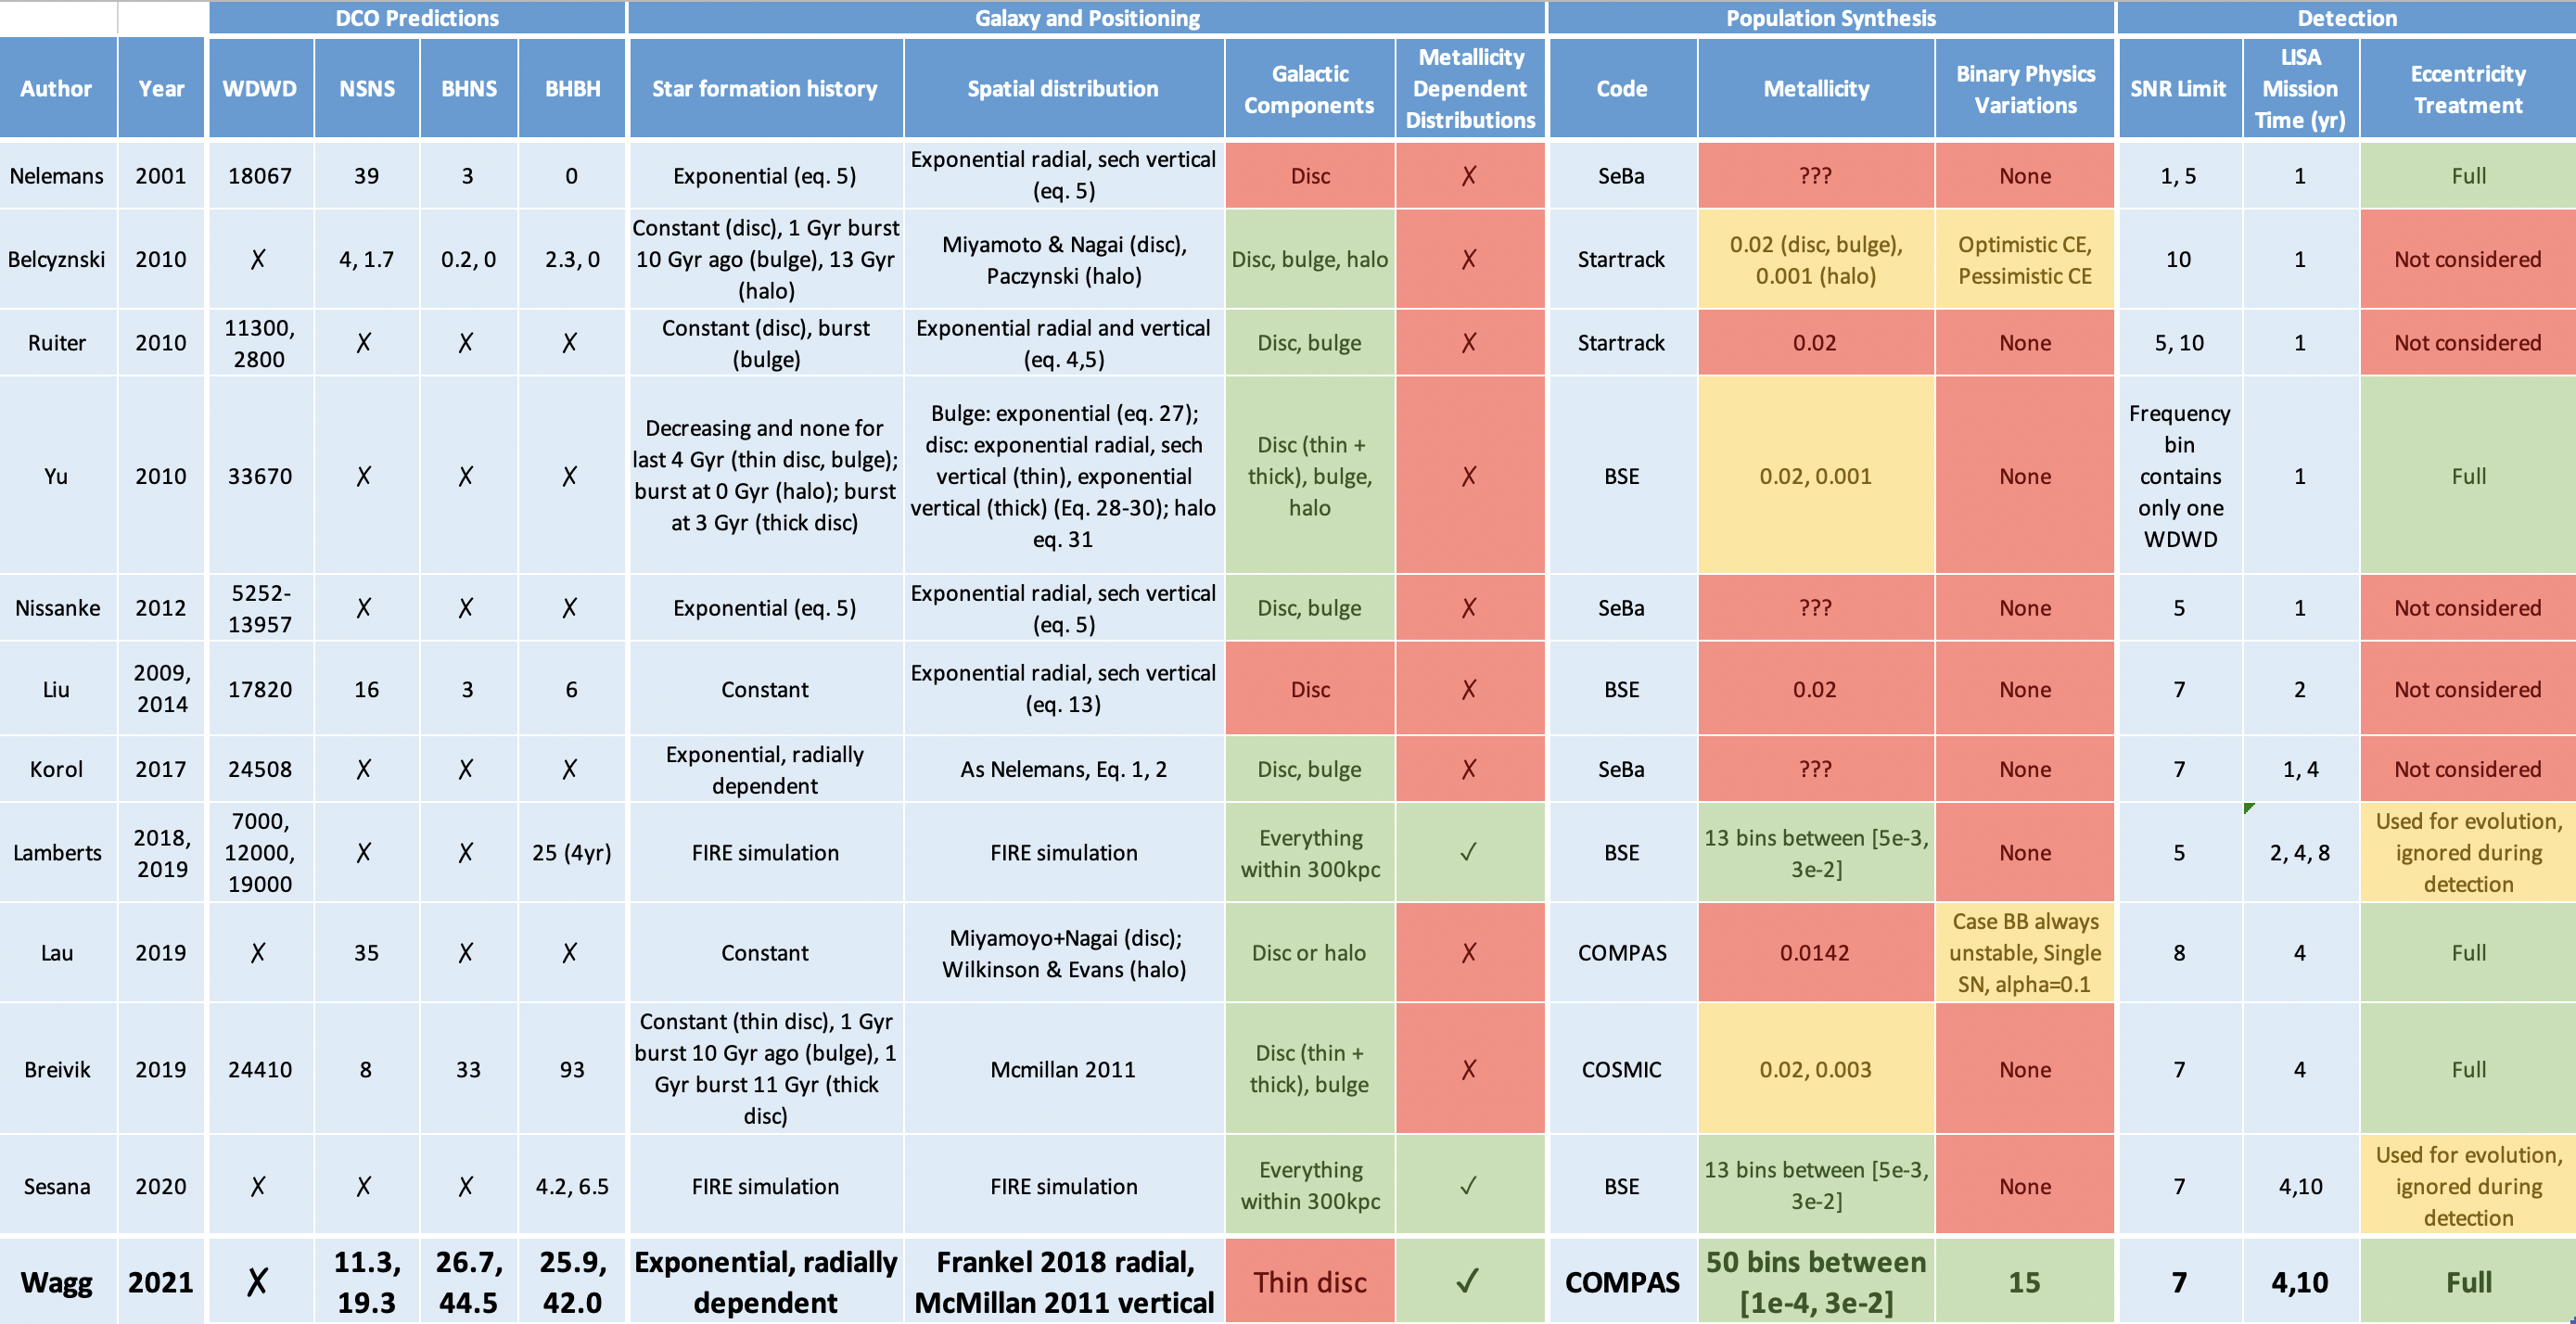
\includegraphics[height=0.95\textheight]{previous_studies.png}
    \caption{A table of previous studies of a similar nature to this work}
    \label{fig:previous_studies}
\end{figure*}

\end{document}

